\vspace{-2pt}
\section{Energy saving policies in action}
\label{sec:energy_savings}
\vspace{-4pt}

Optimizing energy saving in the RAN presents a significant challenge: evaluating the energy saved and its impact on users’ performance~\cite{Tan2022}. 
In this section, we focus on analyzing the energy saving aspect by examining $(i)$~the cell downtime (\ie the amount of time that cells were in sleep mode), and $(ii)$~the energy consumption. We present the impact of energy saving on user performance later in Section~\ref{sec:evaluation-energy_savings}.

\vspace{-2pt}
%\subsection{Capacity Booster Availability}
\subsection{Cell downtime}
\vspace{-2pt}

% \ael{likely, here we need some better glue -- why are we focusing on capacity boosters here?}
%\om{Because the capacity antennas are the antennas affected by the policies, in the discussion section, we are going to discuss a bit about the full region impact and savings.}\ael{sure, but write it down as better glue to the prior section :)}
% \js{I tried to put some glue there :)}

%In the first step of evaluating the benefit of different strategies in terms of energy savings, we focus on quantifying the time that the capacity booster remains in cell sleep (namely, the active policy time interval).  
%Due to the interplay between the policy deployment time window and the ON/OFF cell load thresholds that trigger the policy, the number of capacity boosters that could be impacted and the period these remain in cell sleep varies across strategies. 
%For this, we capture from RAN KPIs the antenna availability, which reports the number of seconds per hour that an antenna was available to provide service.

%Figure~\ref{fig:distribution_downtime_percentage_capacity_booster} shows the distribution of the capacity booster downtime (\ie the active policy time interval), considering the two main deployment time windows, namely, one for the nighttime policies and the other for the full-day policies. 

As mentioned earlier in Section~\ref{subsec:energy-saving-trials} the MNO applies cell sleep strategies only on capacity cells, while coverage cells remain always active. Hence, we measure the impact of the different strategies taking as a reference the \textit{cell downtime}, \ie the amount of time that capacity cells were in sleep mode. For this, we use the cell availability measurements collected from the RAN monitoring infrastructure of the MNO, as described in Section~\ref{data-feeds}. These values allow us to measure the cell downtime with a granularity of seconds.

%Figure~\ref{fig:affected_capacity_booster_average_downtime} shows the percentage of capacity cells that were impacted by a policy undergoing a cell sleep process in at least one instance during the trial week, and the mean downtime of the capacity boosters affected.

%We note that the nighttime strategies are the ones that affected the largest number of capacity boosters, although, as also shown for the shorter period of time, as expected. The full (24/7) energy saving strategies increase the number of antennas included in the energy saving group by the increase of the ON threshold, and also allow antennas to sleep for longer periods of time. 
%It is interesting to note that although the Full-loose strategy has the same ON/OFF thresholds as Night-loose, the fraction of capacity boosters included is smaller. 
%This is due to the fact that a fraction of capacity boosters were sleeping before the nighttime deployment time window, reducing the possibility of switching off as many cells as the Night-loose strategy, while meeting the end-user demand. 

Figure~\ref{fig:affected_capacity_booster_average_downtime} shows the percentage of capacity cells affected by each of the strategies, \ie cells that entered at least once into sleep mode over the weekly trial periods, and the average percent downtime of these cells. Overall, the strategies that operate only over the nighttime (Night-loose and Night-strict) exhibit significantly less downtime, while the number of cells affected (at least once) is slightly larger. Full-day strategies (24h) affect more cells as the strategy is more aggressive (\ie higher ON/OFF thresholds are higher).

The figure also reports the average and standard deviation of the total percent of the time during which cells remain in sleep mode for each strategy. This statistic grows with the aggressiveness of the strategy. For example, in the Dense region, we observe a rise in the mean downtime from 40.6\% with the Full-loose strategy (5/10 for ON/OFF load thresholds) to 51.5\% with the Full-strict strategy (10/15\% for ON/OFF thresholds). It is interesting to note that although the Full-loose strategy has the same ON/OFF load thresholds as the Night-loose, the fraction of capacity cells affected is slightly larger in the latter. Upon verifying with the operation team of the MNO, this was, in fact, a symptom of misbehavior by the nighttime energy saving strategies, where the cells were failing to wake up from cell sleep, even when the load was reaching levels above the OFF threshold. Nevertheless, the results are still consistent when we look at the average cell downtime. The mean downtime increased by $25.0\%$ and $36.3\%$ in the Dense and Sparse regions, respectively, when comparing the Full-strict with the Night-loose strategies.
% \ael{in fact, another explanation here is that the strategy is simply not working correctly, and some of the cells never wake up -- this, in fact, is much more likely than the fact that the radio team simply over-dimensioned the deployment :)}\jo{also, probably that sentence will be one that Clive won't like in a public paper.}
%In other words, in some regions the network may seem to be over-dimensioned, while in others all cells are critical towards meeting the demand in their area.
%Upon verifying with operations, this was, in fact, a symptom of a mis-behaving energy saving strategy, where the cells were failing to wake up from cell sleep, even when the load was reaching levels above the OFF threshold.
% \js{Does it sound convincing ??}


\begin{figure}[!t]
    \centering
    \subfloat{
\includegraphics[width=.58\columnwidth]{images/availability/affected_and_downtime/legend.pdf}}
    
    % \cesntering
    \subfloat[Dense region]{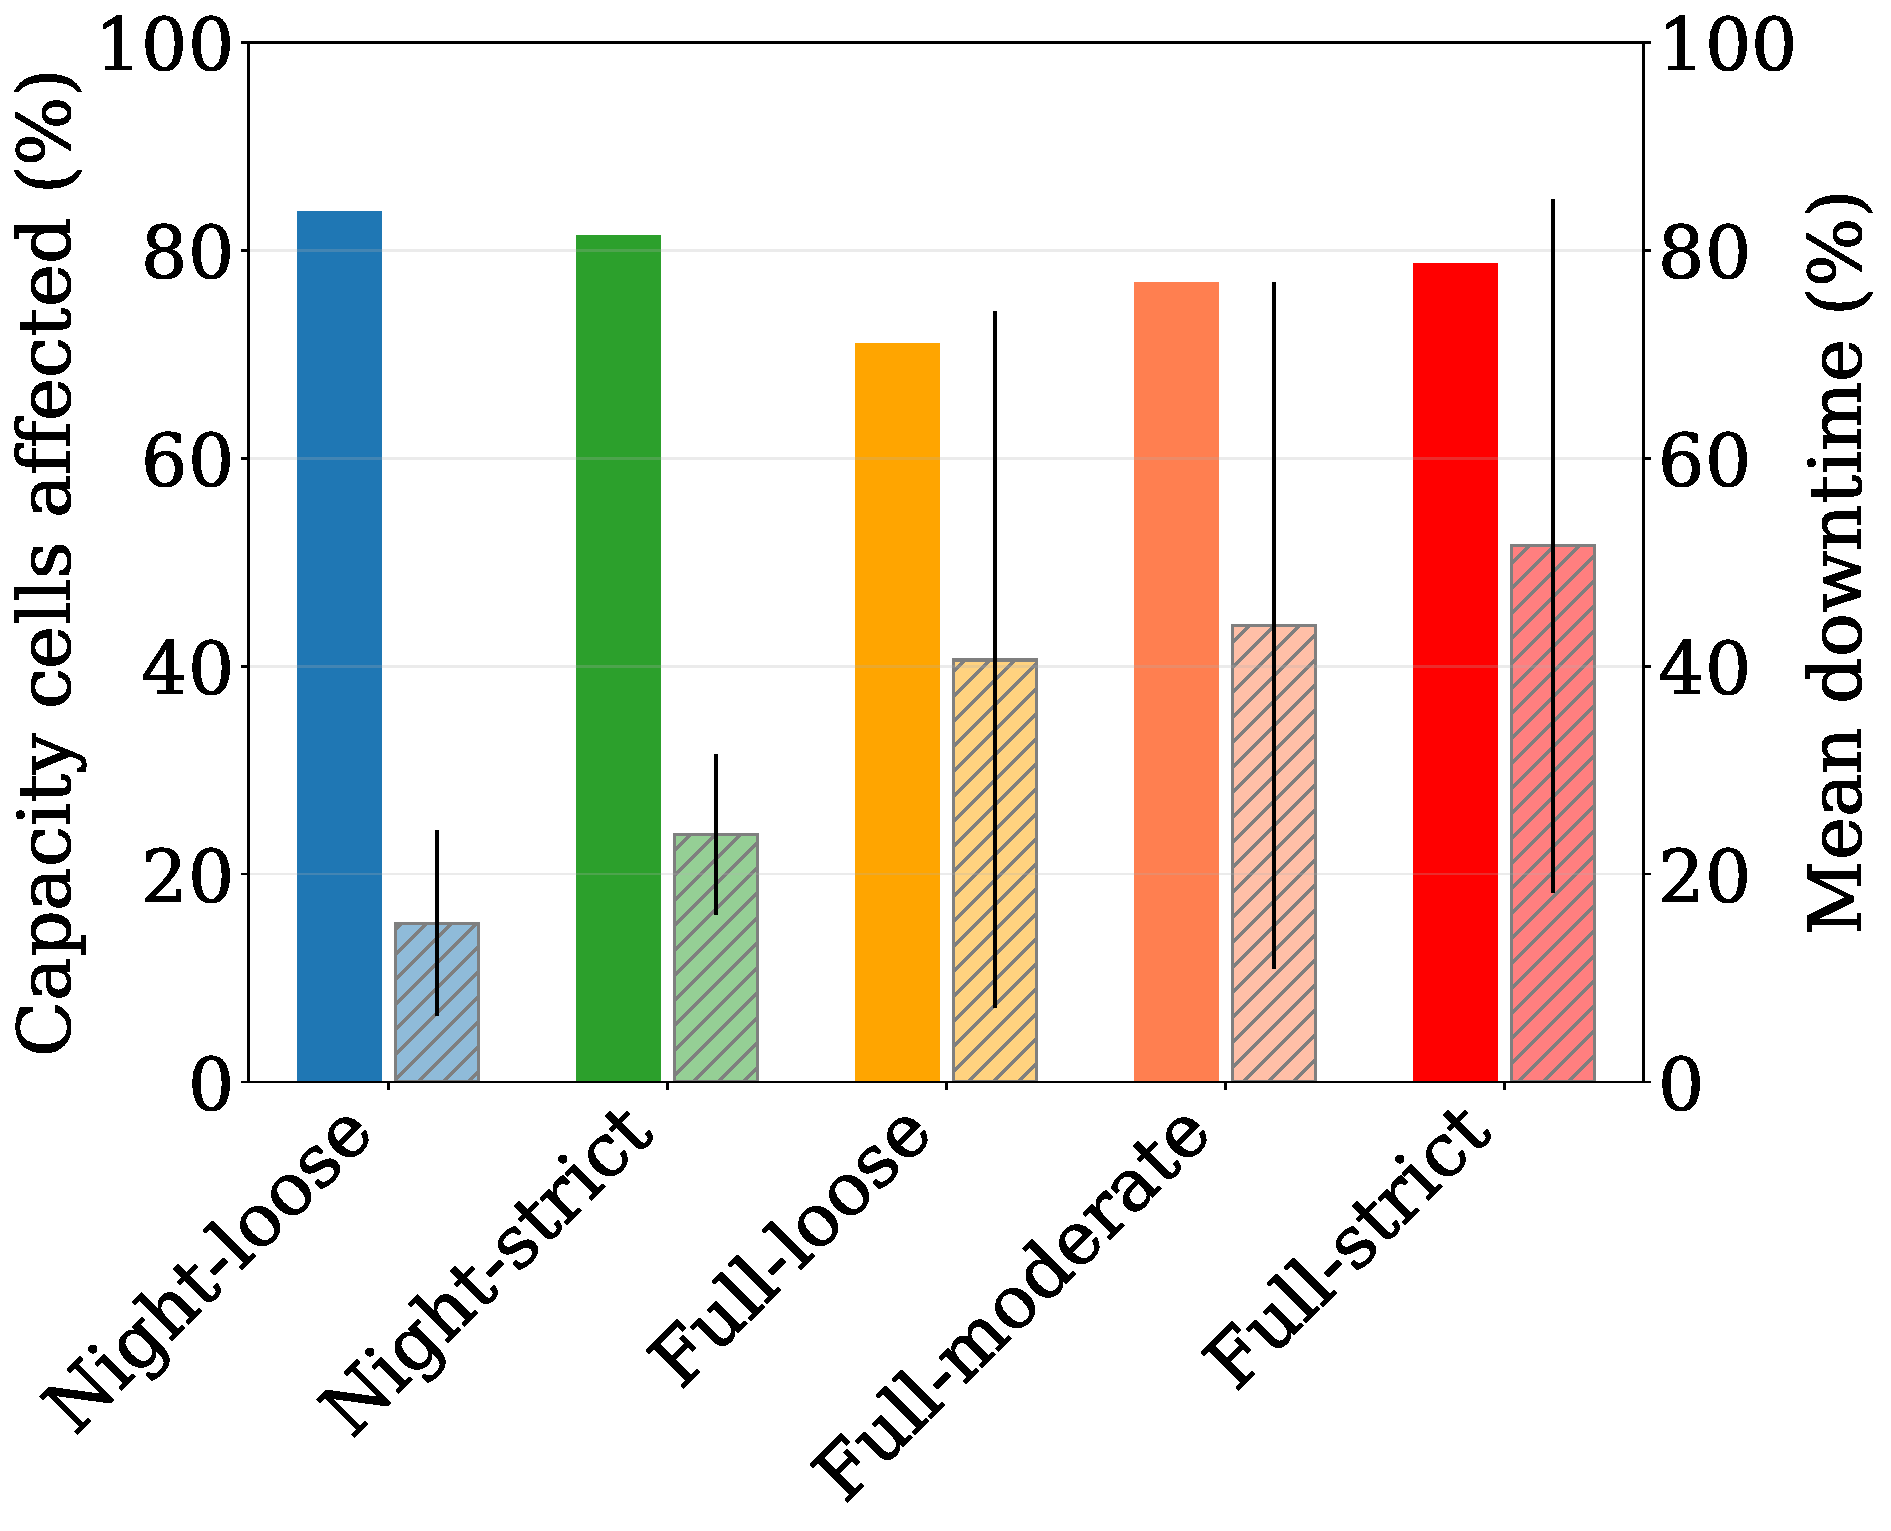
\includegraphics[width=.5\columnwidth]{images/availability/affected_and_downtime/fraction_affected_antennas_and_up_time_north_london.pdf}}
    % \hspace{3pt}
    \subfloat[Sparse region]{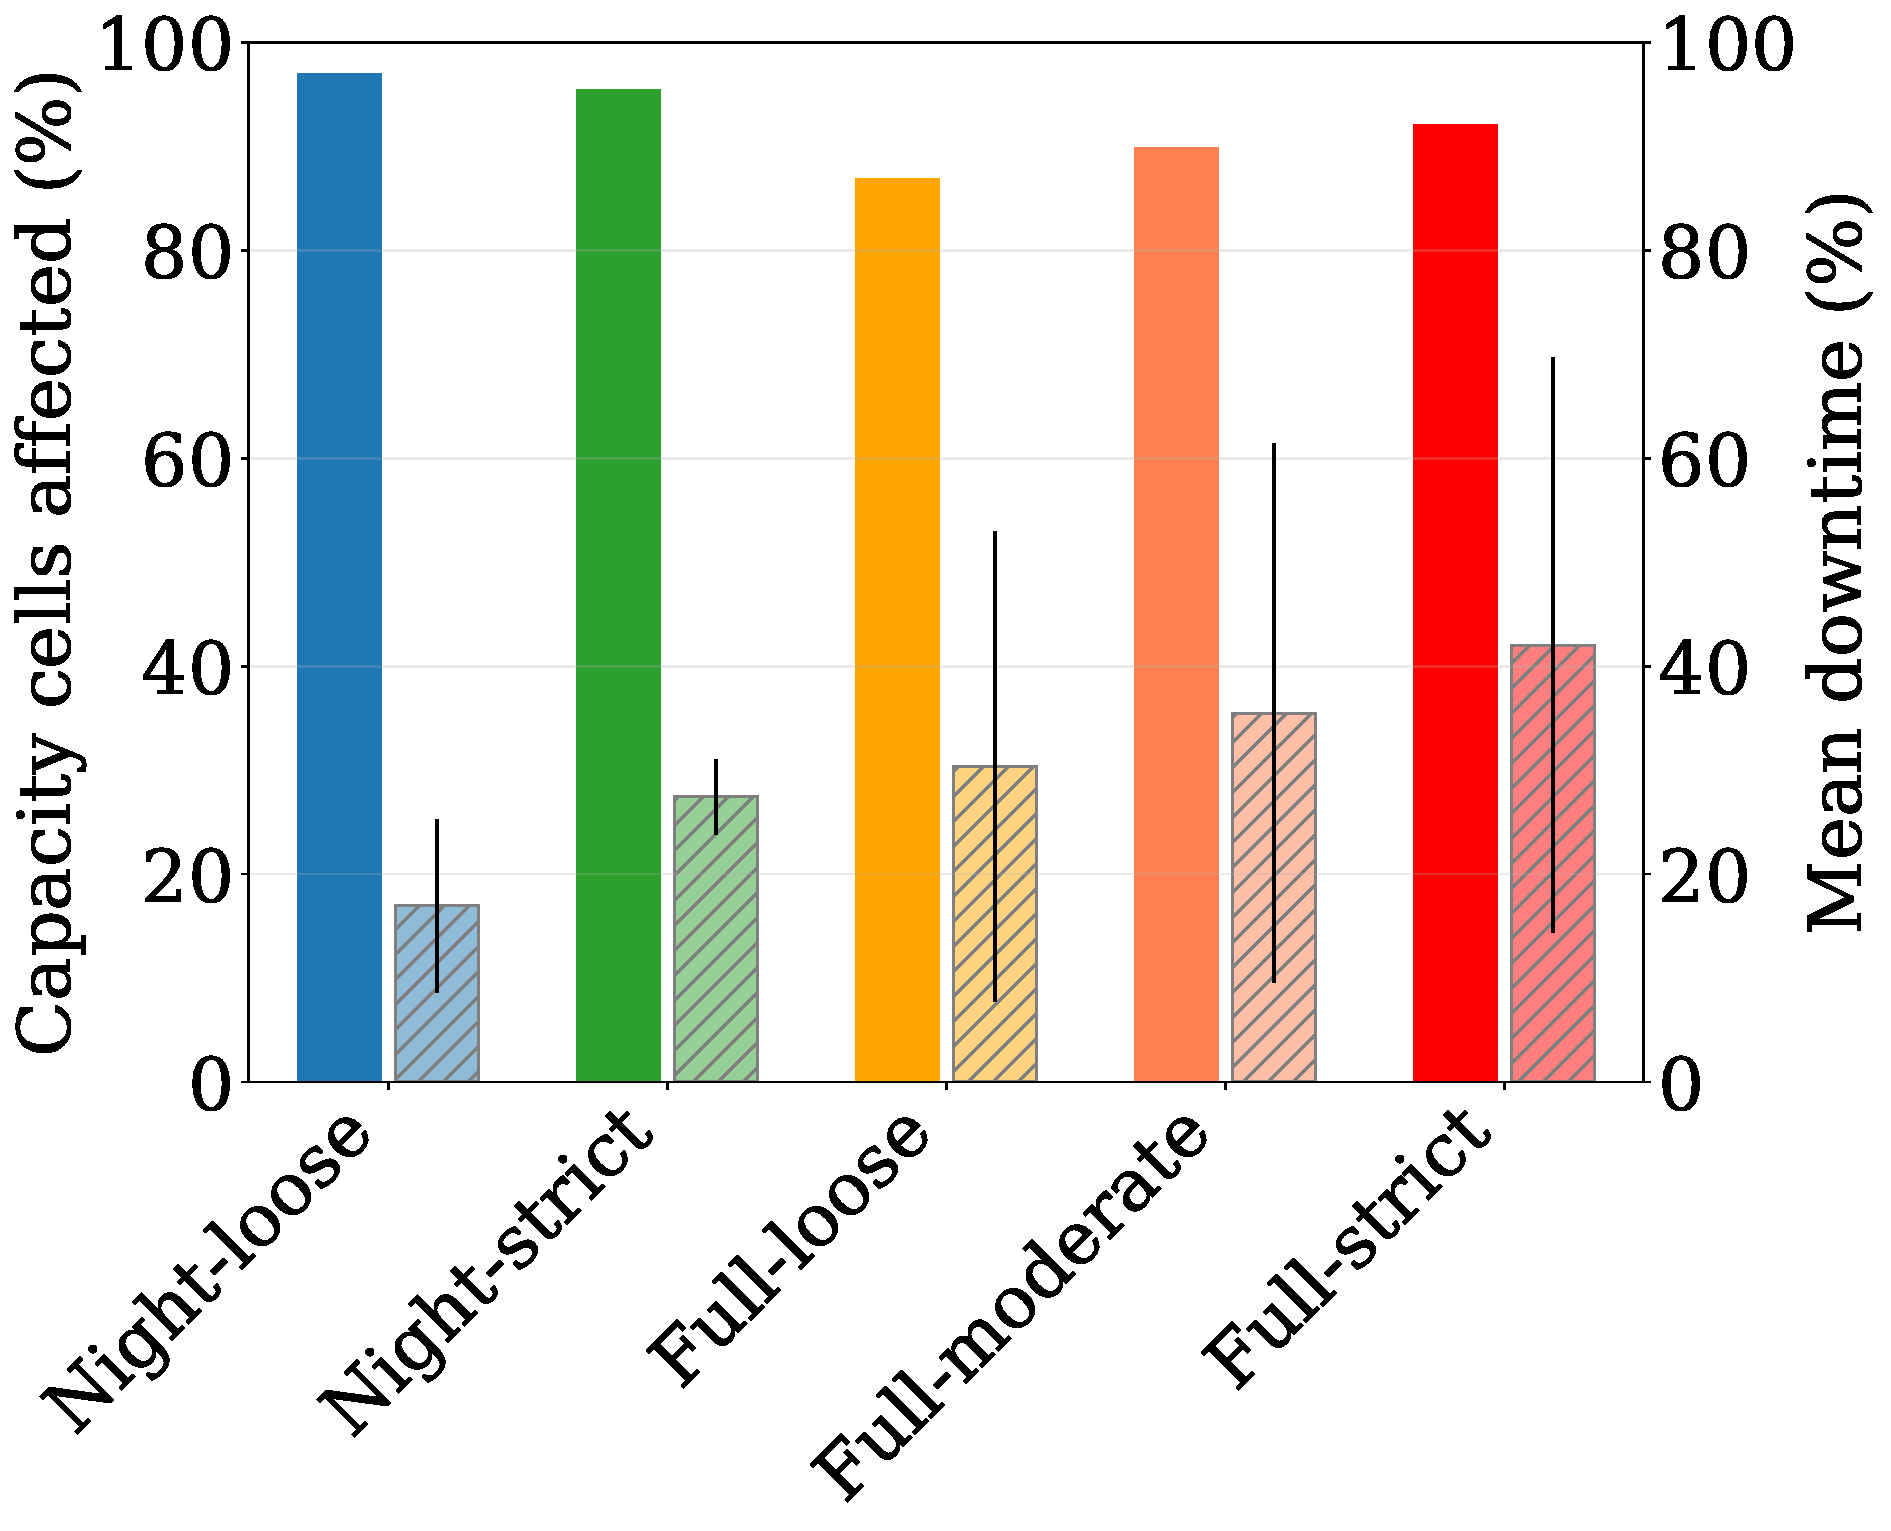
\includegraphics[width=.5\columnwidth]{images/availability/affected_and_downtime/fraction_affected_antennas_and_up_time_southeast.pdf}}
    \vspace{-4pt}
    \caption{\small Percentage of capacity cells affected by the energy saving strategies and their corresponding mean downtime (\ie the percentage of time that cells were in sleep mode). Error bars show the standard deviation across all the measured capacity cells.
    }\label{fig:affected_capacity_booster_average_downtime}
    \vspace{-15pt}
\end{figure}

To further dig into the behavior of the different strategies, Figure~\ref{fig:distribution_downtime_percentage_capacity_booster} shows the distribution of cell-level downtime. We observe that policies operating only during nighttime exhibit some inconsistency in their distribution across the two regions, likely due to the issue mentioned above. In contrast, full-day strategies show more consistent behavior across cells. For these strategies, a main takeaway is that as the policy becomes more aggressive (\eg Full-strict), cells display a more heterogeneous behavior, 
% \jo{not clear what you want to say here}
observing sparser distributions as the strategy becomes stricter, \eg more cells experience considerably higher downtime, suggesting that these strategies even keep a small portion of cells inactive for most of the time  (see right part of the distributions). While these less-conservative behaviors can help save more energy, they may also have some impact on end-user performance --and aspect that we further investigate in Section~\ref{sec:evaluation-energy_savings}.
%Moreover, we extract two main takeaways: ($i$)~A fraction of the capacity cells %included in the energy saving group does not undergo cell sleep (\ie cells that fall at the left of the distribution), and 
%($ii$)~a different fraction remains in sleep mode during the full deployment time window, highlighting the heterogeneity of the end-user demand and traffic load. 



\begin{figure}[!t]
    \centering
    \subfloat{
\includegraphics[width=.8\columnwidth]{images/availability/distribution/legend.pdf}}
    \setcounter{subfigure}{0}
    
    \subfloat[Dense region]{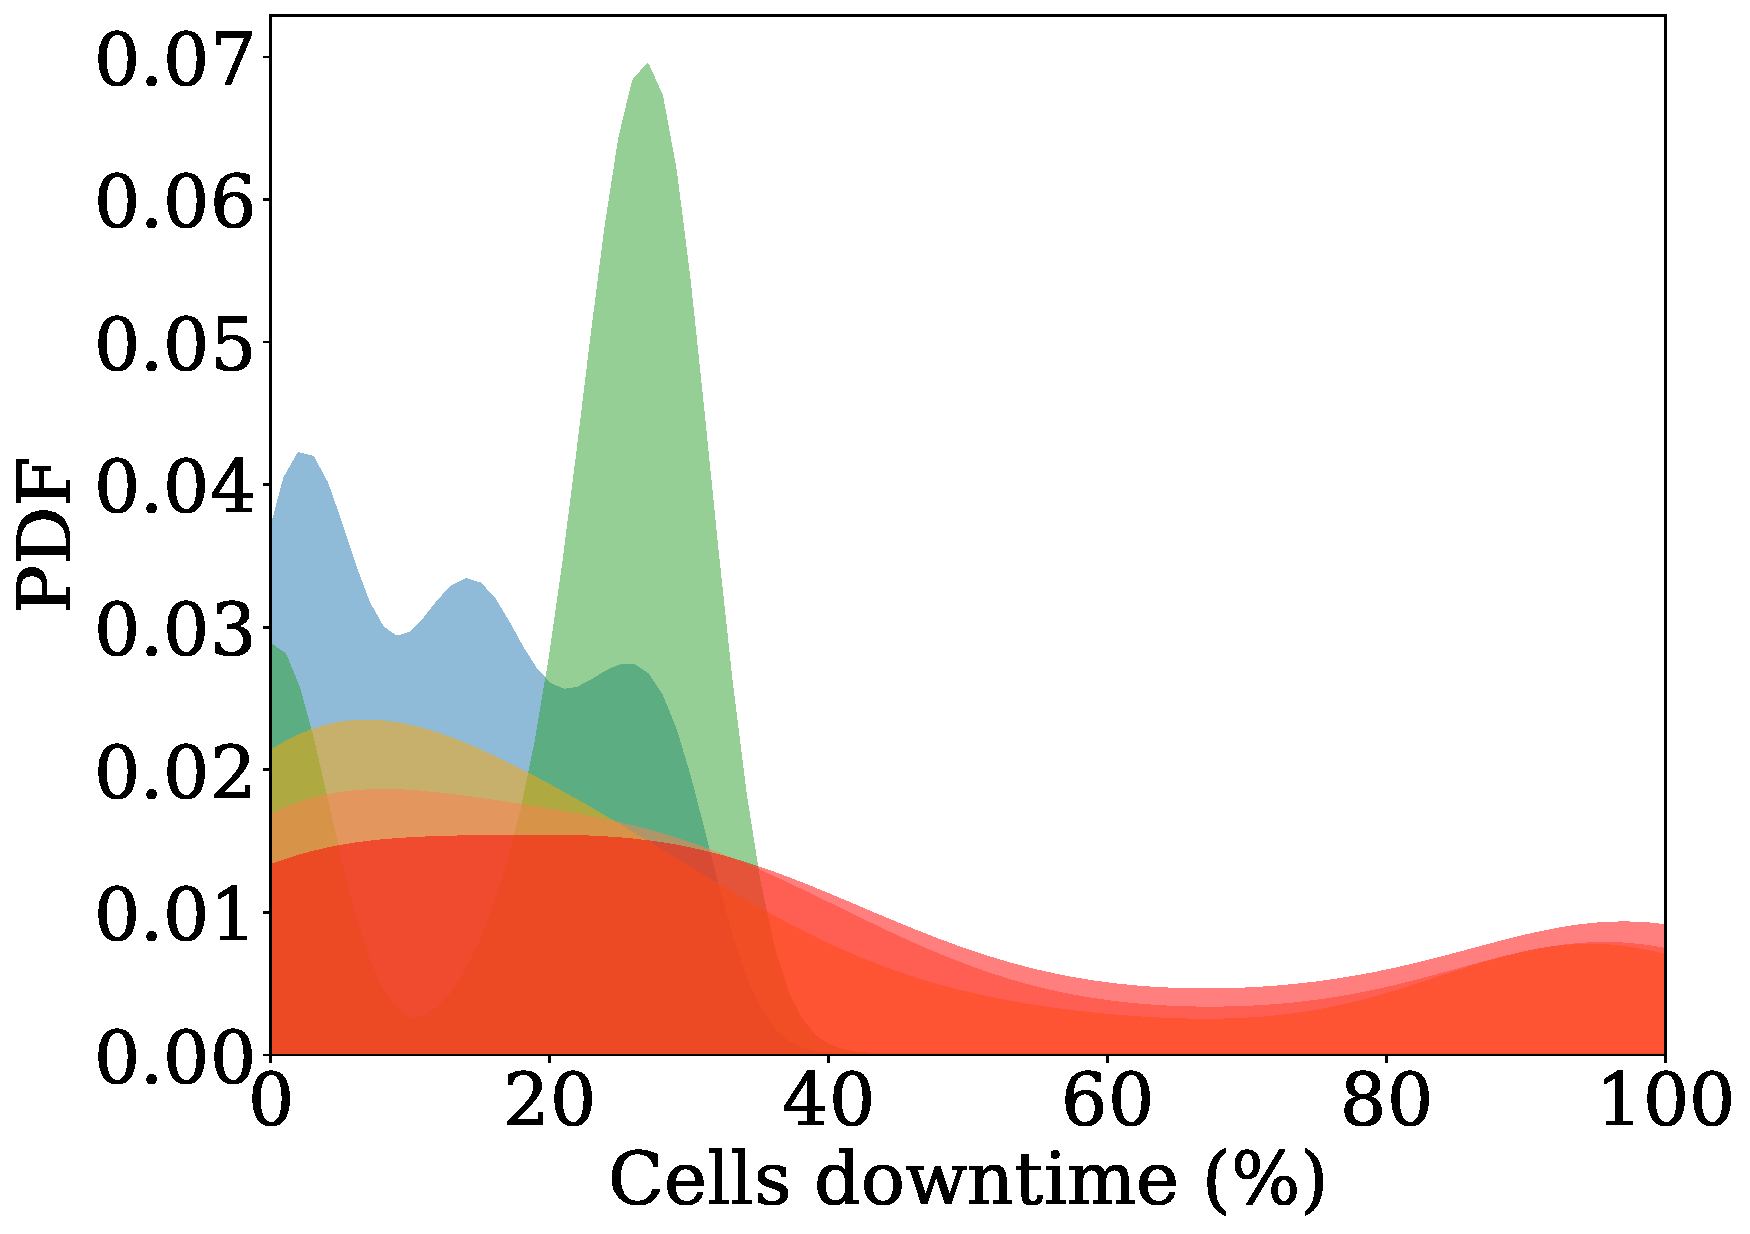
\includegraphics[width=.475\columnwidth]{images/availability/distribution/dist_avail_capacity_boosters_north_london.pdf}}
    % \hspace{5pt}
    \subfloat[Sparse region]{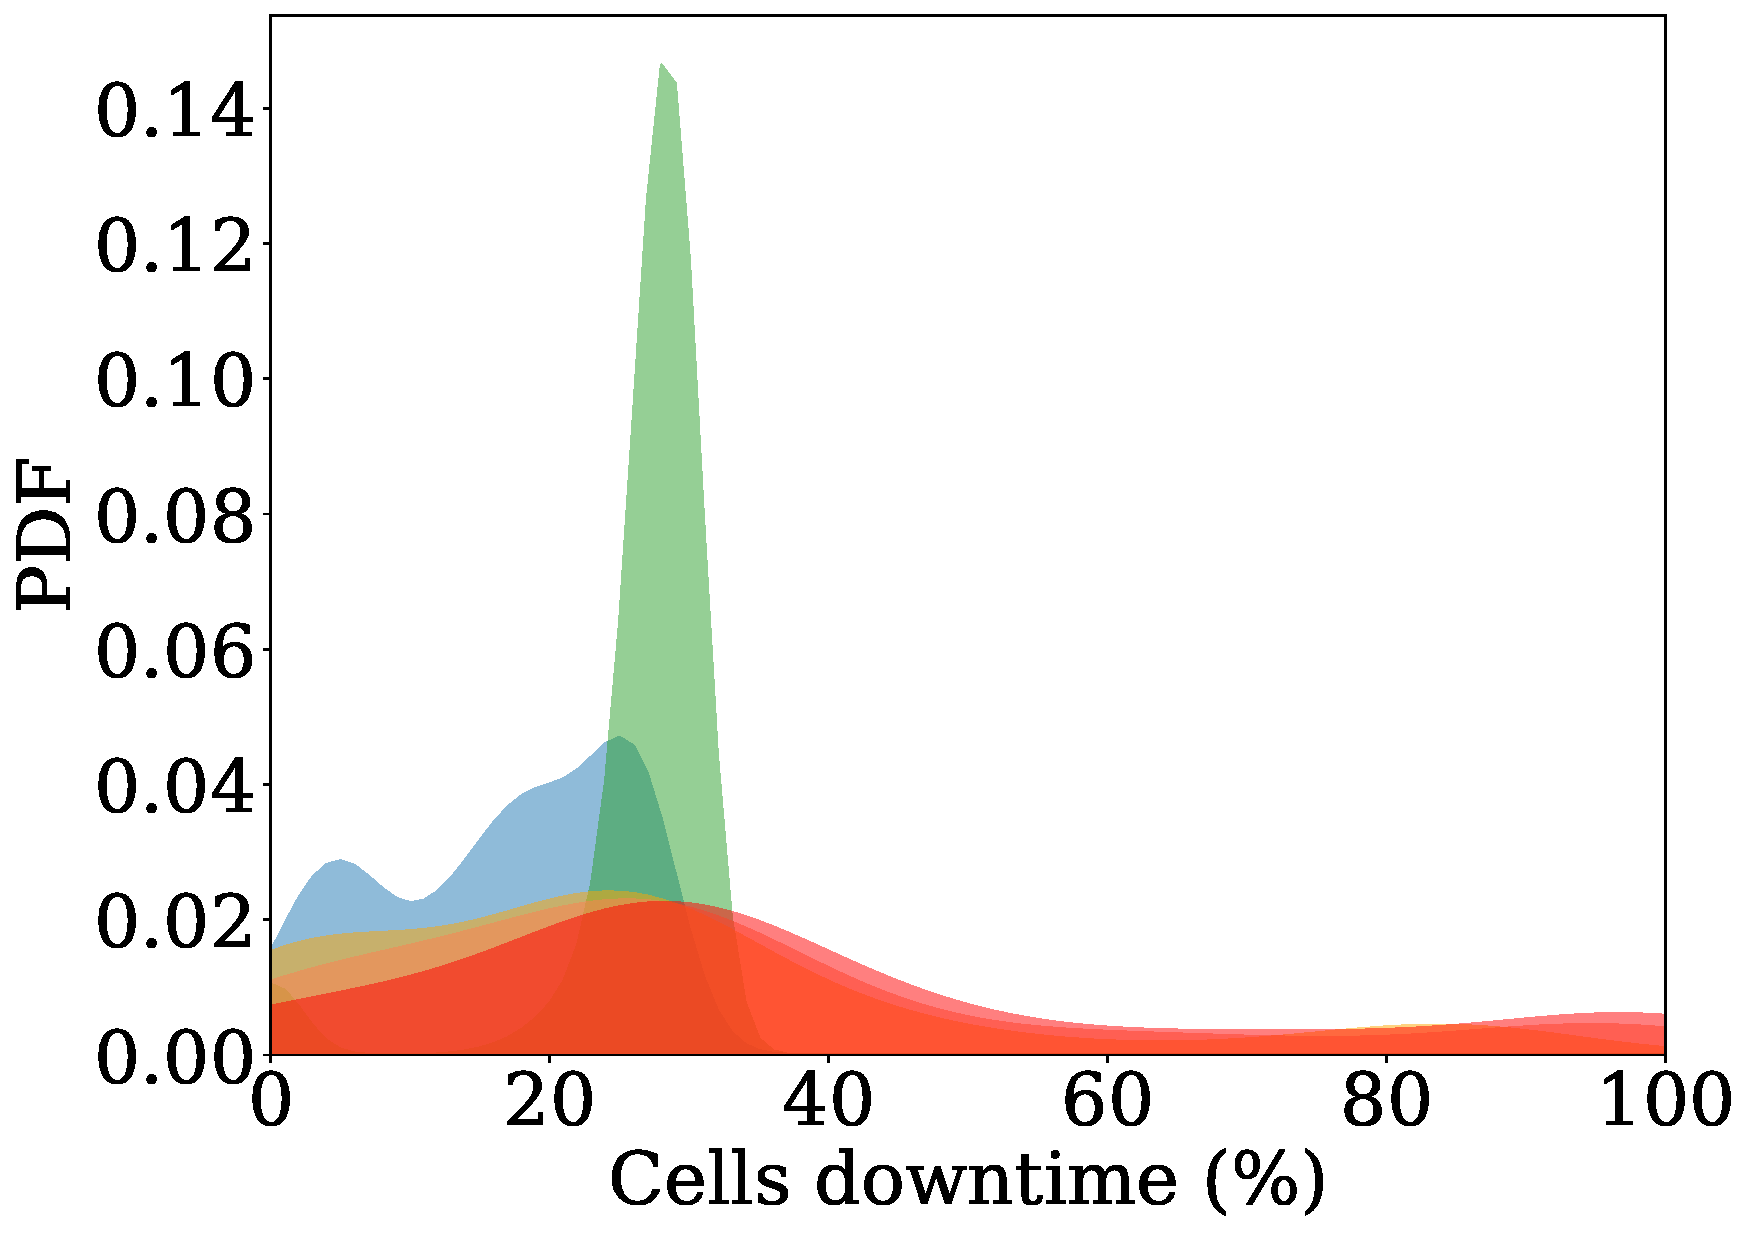
\includegraphics[width=.475\columnwidth]{images/availability/distribution/dist_avail_capacity_boosters_southeast.pdf}}
    \vspace{-4pt}
    \caption{\small Distribution of cell-level downtime (in \%) of capacity cells for the energy saving strategies tested by the MNO.
    % \om{working on Marco's version without the overlap}
    % \js{change X label to "Cell downtime (\%)"}
    \label{fig:distribution_downtime_percentage_capacity_booster}}
    \vspace{-15pt}
\end{figure}

We complete the characterization of the downtime by looking at the temporal evolution of the amount of time that cells spend in sleep mode over different moments of the day. Figure~\ref{fig:time_series_mean_downtime} shows the hourly evolution of the mean downtime of capacity cells across all the different strategies, each tested for a one-week period. Overall, we observe clear day-night patterns, where all strategies benefit from the low traffic load over the night period, as shown by downtime peaks occurring during the nighttime for all strategies. Likewise, full-day strategies consistently show increased downtime as they become stricter, both during the day (valleys of the curve) and at night (peaks of the curve). In addition, the Night-strict strategy shows longer sustained peak periods during the night, this is mainly due to the higher OFF loading threshold (20\% PRB utilization) which forces the cells to remain in sleep mode for longer periods of time while the policy is active.

%Night strategies exhibit two different behaviors: $(i)$ Night-strict forces cells to stay on for longer periods of time due not only to the higher ON load threshold (10\% of PRB utilization), $(i)$ also to the higher gap with respect to the OFF load threshold (20\% of PRB utilization). 
%Also, we note that the mean downtime increased by $25\%$ and $36.29\%$ in the Dense and Sparse regions, respectively, when comparing the Full-strict with the Night-loose strategies.
% \ael{how much? quantify this} for the full-day strategies.

\begin{figure*}[!t]
    \centering
    \subfloat{
\includegraphics[width=.8\textwidth]{images/availability/time_series/legend.pdf}}
    \setcounter{subfigure}{0}
    
    \vspace*{-10pt}
    \subfloat{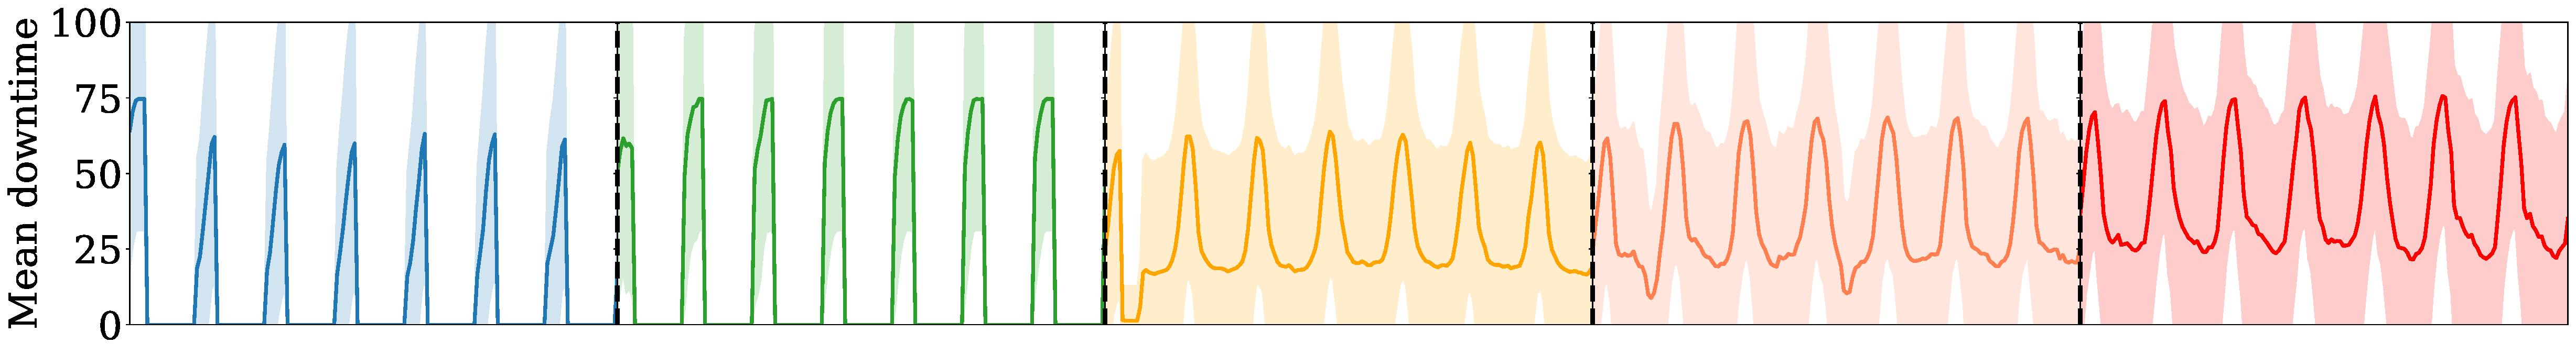
\includegraphics[width=.95\textwidth]{images/availability/time_series/capacity_booster_downtime_timeseries_north_london_axes_weeks.pdf}}

    \subfloat{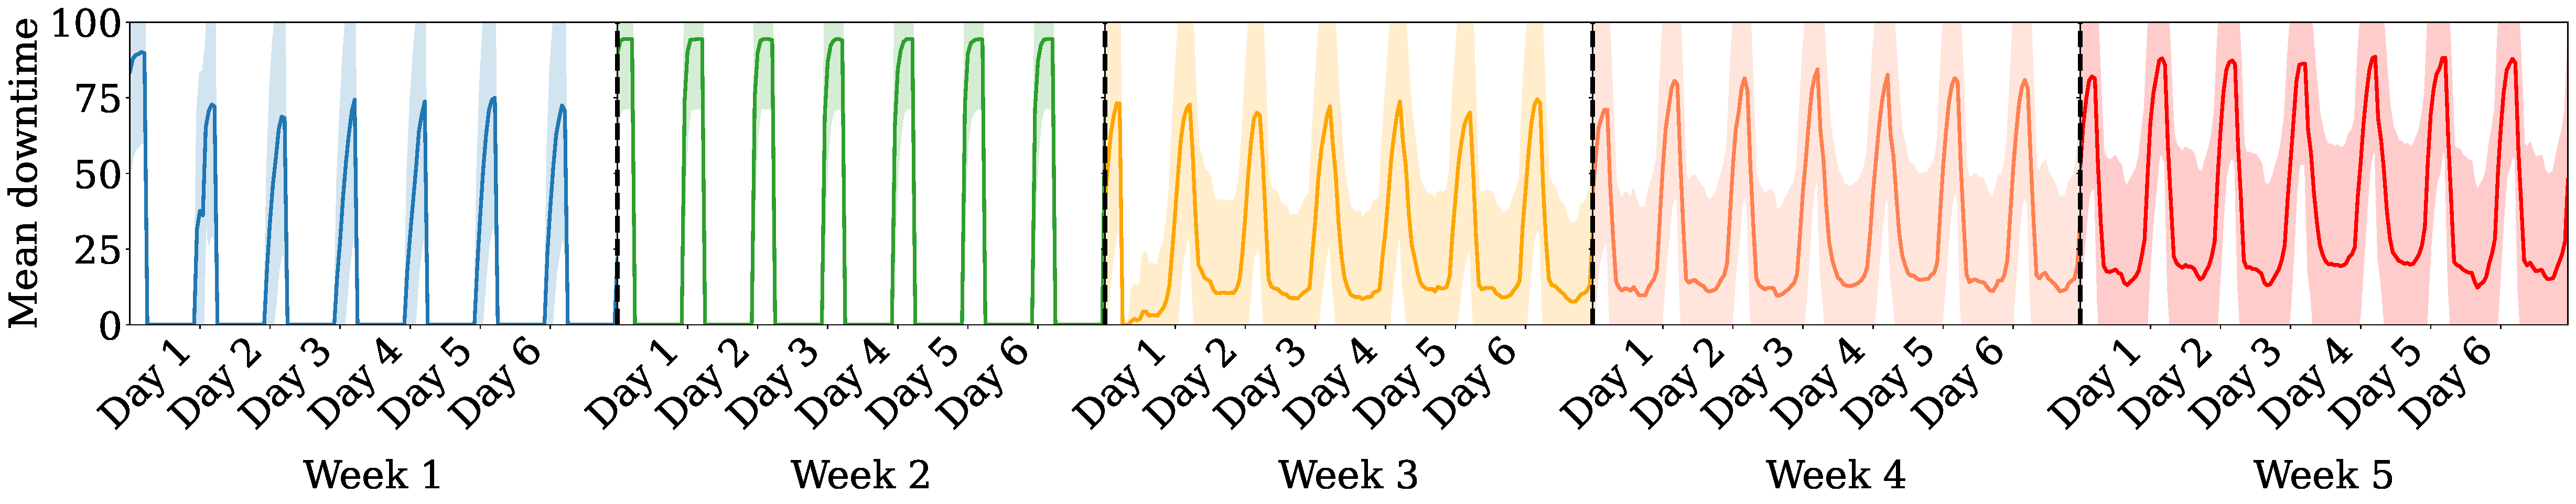
\includegraphics[width=.95\textwidth]{images/availability/time_series/capacity_booster_downtime_timeseries_southeast_axes_weeks.pdf}}
    \vspace{-4pt}
    \caption{\small Hourly time series of the mean cell downtime; Top: Dense region, and bottom: Sparse region. Shades indicate the standard deviation of the downtime distribution across all capacity cells. 
    % \js{@Orlando: Is it the std. dev. or the min/max?}\om{the std over all the capacity booster downtime in that hour}
    }
    \label{fig:time_series_mean_downtime}
    \vspace{-15pt}
\end{figure*}

\vspace{-2pt}
\subsection{Energy consumption}
\vspace{-2pt}

In this section, we translate the cell downtime into actual energy savings. 
%A mobile cellular network has several energy-demanding components, such as the cloud, physical link, base station, and antennas. 
For this, we focus on the energy consumed at the cell level, and rely on an operational energy consumption model that estimates the energy usage of a full base station\cite{energy_consumption_formula}. The energy consumption model is 
% mathematically 
expressed in Eq.~\ref{eq:energy_consumption_base_station} as:
%While specific parameters remain confidential, the  is shown . 
\begin{equation}
    E_{BS} = E_{BBU} + \sum_{i} E^{i}_{RRU},
    \label{eq:energy_consumption_base_station}
\end{equation}
where $E_{BBU}$ accounts for the energy consumed by the processing of baseband signals and remains relatively constant and not affected by traffic load, while $E^{i}_{RRU}$ is the cost associated with the radio unit and expressed as follows:
\begin{equation}
    E_{RRU} = \alpha \cdot R_{PRB} \cdot P_{m} + \gamma,
    \label{eq:energy_consumption_radio_unit}
\end{equation}
where  $R_{PRB}$ represents the fraction of PRBs used (\ie the load), and $P_{m}$ denotes the maximum transmit power of the antenna (set by the operator). $\alpha$ and $\gamma$ account for the power amplifier efficiency and fixed circuit power, respectively, and are specific to the antenna type, frequency, and number of transmitters.\footnote{For confidentiality reasons we cannot disclose the values of the model parameters used in the two formulas, which were empirically obtained.} 

In the analyzed MNO trials, coverage cells remain always active, hence base stations never turn off. This means that the $E_{BBU}$ element of the energy consumption model remains always active %relatively constant 
for all base stations.
%With energy-saving strategies that integrate the \textit{cell sleep} policy, base stations never turned off completely; coverage antennas remain available in order to provide coverage, hence the $E_{BBU}$ element of the energy consumption model remains %relatively constant 
%for all base stations. %, and it is not affected by the cell sleeping policy. Henceforth, we focus 
Consequently, energy savings are only reflected on the $E_{RRU}$ component: when a cell enters in sleep mode the consumption related to the radio unit drops to zero according to the energy consumption model (\ie $E_{RRU}$ = 0 kWh). 
% \js{Double check this description. @Orlando: does $\gamma$ drop to zero in this case?}\om{yes it does, coz there are some capacity cell that are always off.}

\begin{figure}    
    \centering
    \subfloat[Capacity cells]{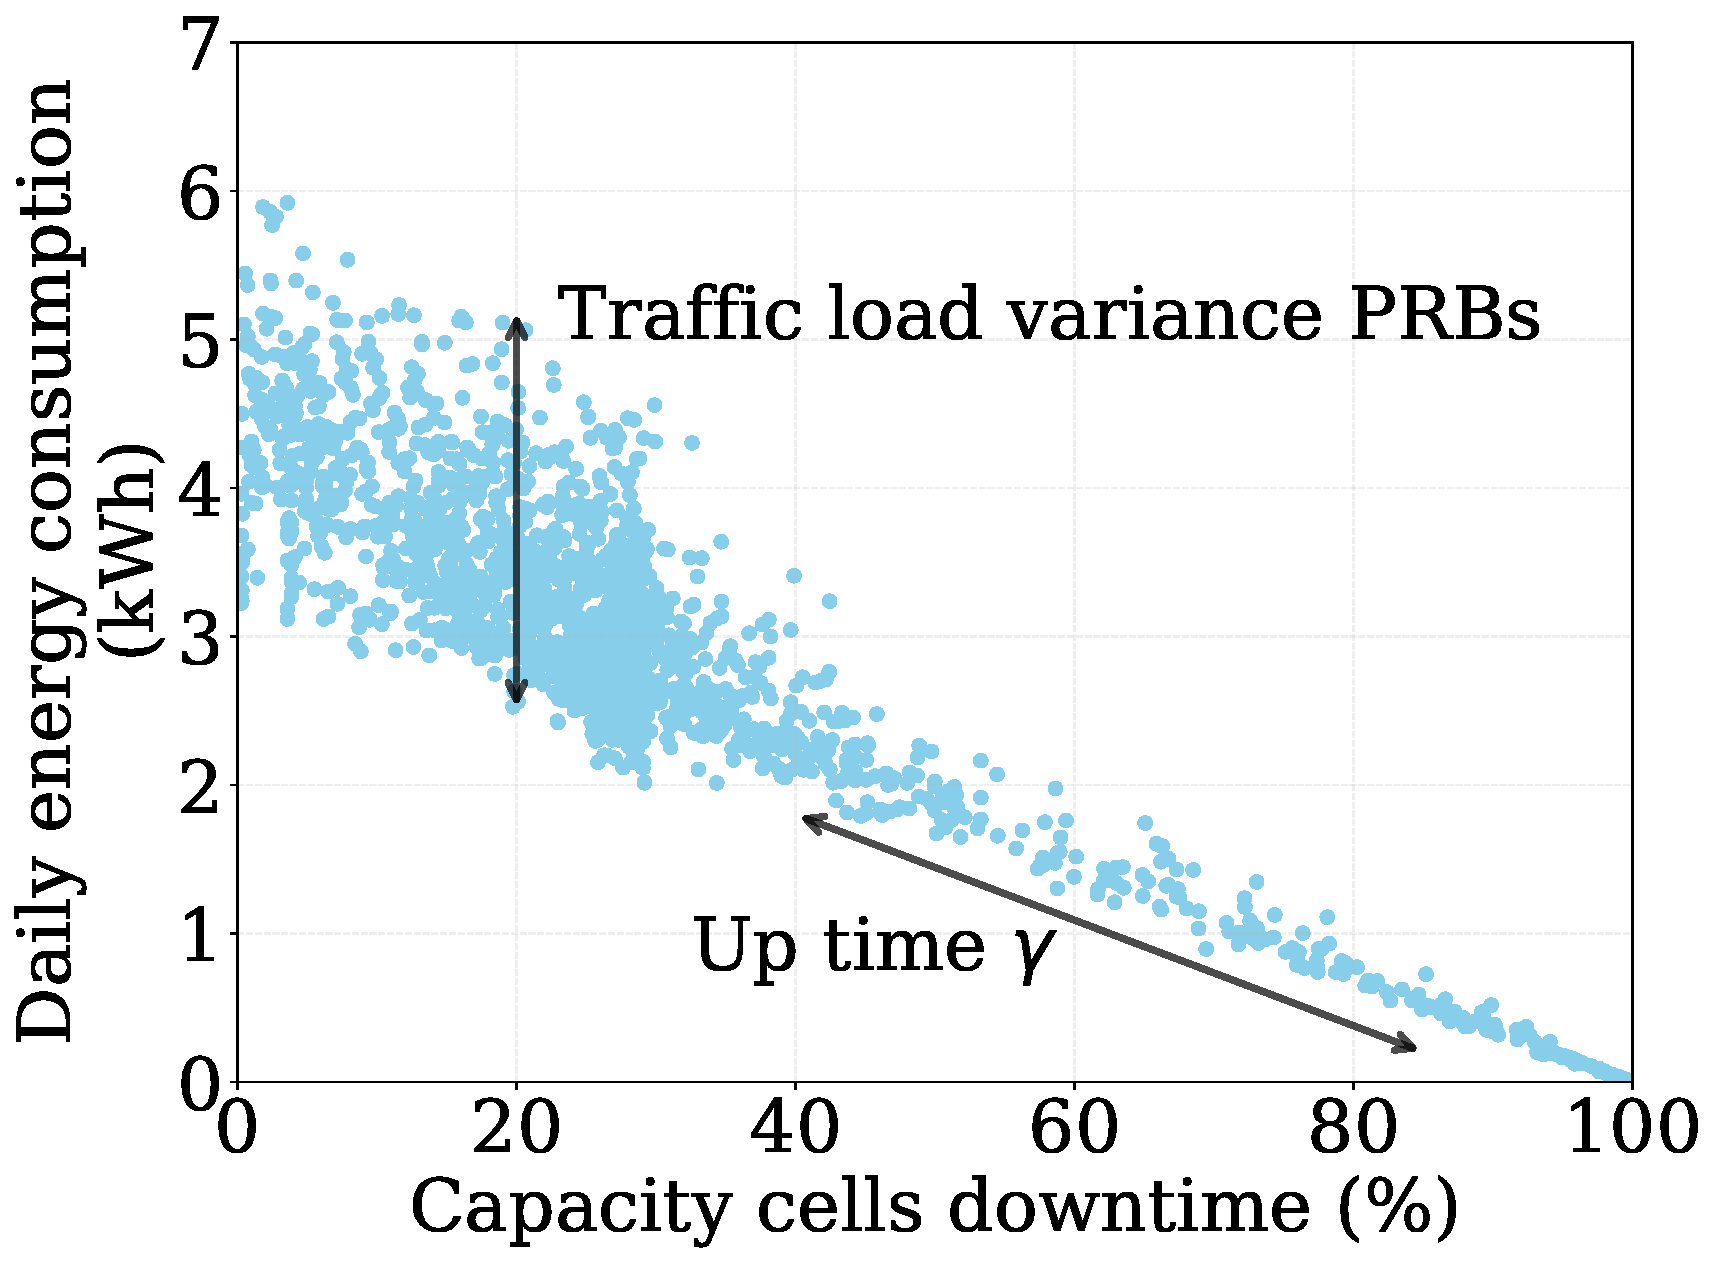
\includegraphics[width=.5\columnwidth]{images/energy/distribution_and_model/avail_vs_energy_consumption.pdf}\vspace{5pt}\label{subfig:energy_consumption_parameter}}
    % \hspace{5pt}
    \subfloat[Coverage cells]{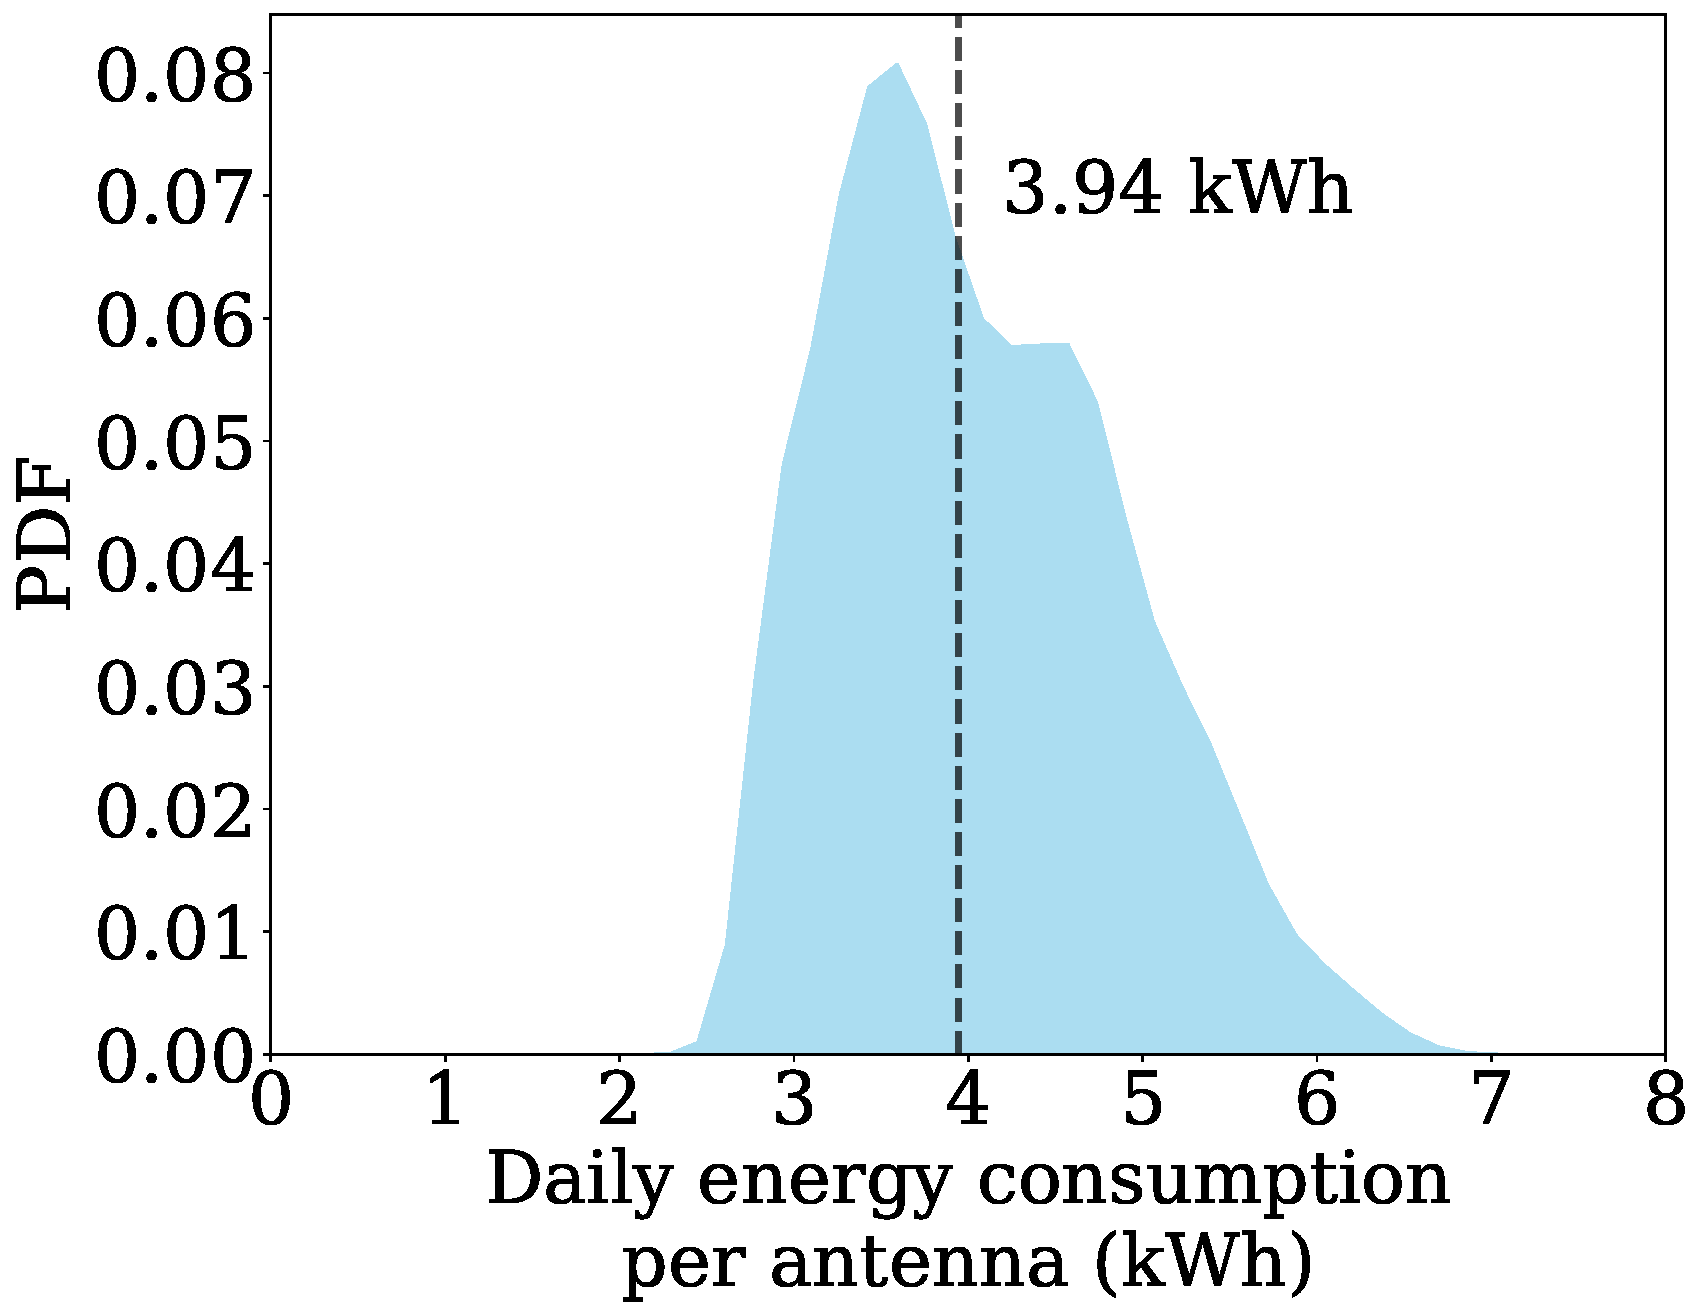
\includegraphics[width=.5\columnwidth]{images/energy/distribution_and_model/energy_consumption.pdf}\label{subfig:energy_consumption_distribution}}
    \caption{\small Energy consumption of Radio units~($E_{RRU}$).
    }\label{fig:daily_energy_consumption_model}
    \vspace{-15pt}
\end{figure}

Figure~\ref{subfig:energy_consumption_parameter} shows the relationship between the cell downtime and the corresponding cell-level energy consumption on daily intervals for all capacity cells in the two studied regions. Since measurements are at the cell level, we show only energy consumption due to the $E_{RRU}$ component; note that $E_{BBU}$ applies at the base station level and does not depend on cell downtime. Here we observe that $\gamma$ produces a constant contribution to the energy consumption (see Eq.~\ref{eq:energy_consumption_radio_unit}), which is proportional to the time that the cell is active (\ie~inversely proportional to the downtime). Likewise, traffic load plays a crucial role in energy consumption, which affects the $R_{PRB}$ component in Eq.~\ref{eq:energy_consumption_radio_unit}. We would expect that capacity cells that go into cell sleep more often (\ie higher downtime) consistently handle low daily traffic loads. This is reflected in the results, where we see that energy consumption experiences greater variability as cell uptime becomes longer (left part). This is explained by the increasing heterogeneity of daily traffic loads on those antennas that remain active for a longer time period.
To complement our analysis, we show in Figure~\ref{subfig:energy_consumption_distribution} the average daily energy consumption per antenna for all coverage cells --~which remain active all day. The distribution shows that energy consumption also varies significantly among cells of this type, with a median consumption of $3.94$ kWh.
% \js{@Orlando: give more details here. Where and how do you use it?}

% \begin{figure}
%     \RaggedLeft
%     \subfloat{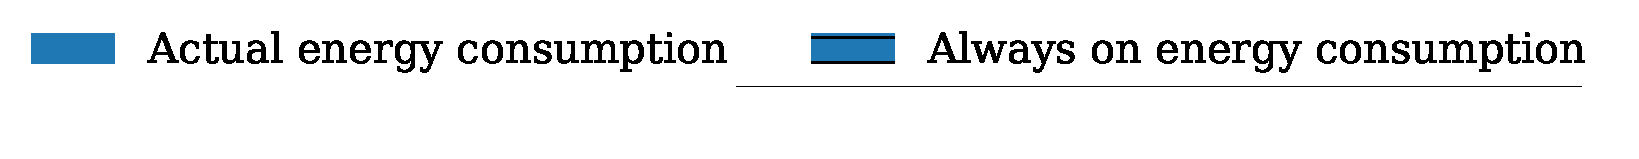
\includegraphics[width=.9\columnwidth]{images/energy/energy_saving/capacity_booster/energy_consumption_actual_and_benchmark_legend.pdf}}
%     \setcounter{subfigure}{0}
%     \centering
%     \subfloat[Urban region]{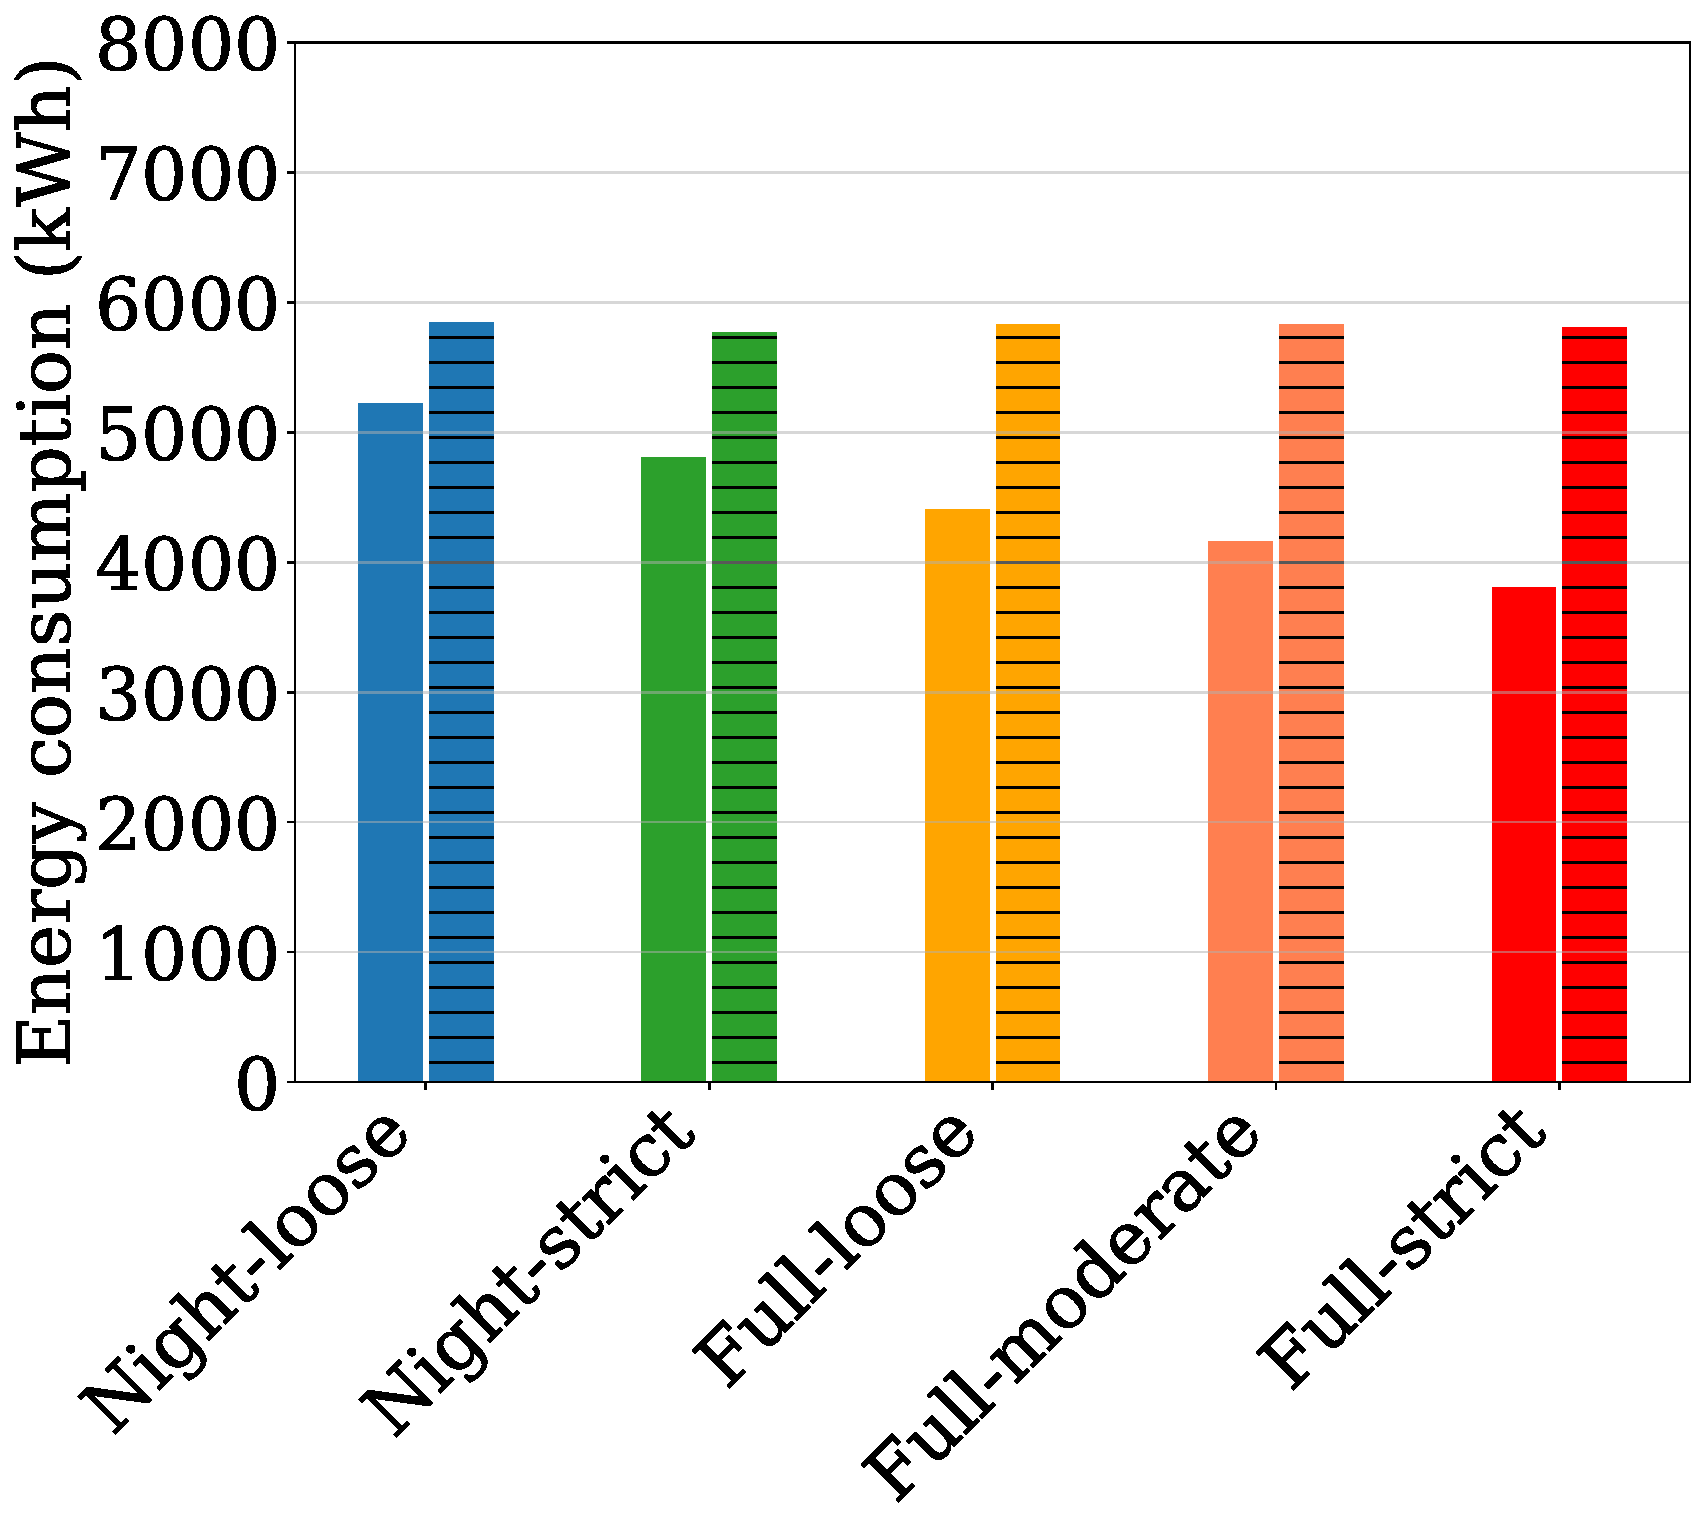
\includegraphics[width=.5\columnwidth]{images/energy/energy_saving/capacity_booster/energy_consumption_actual_and_benchmark_north_london.pdf}}
%     \subfloat[Rural region]{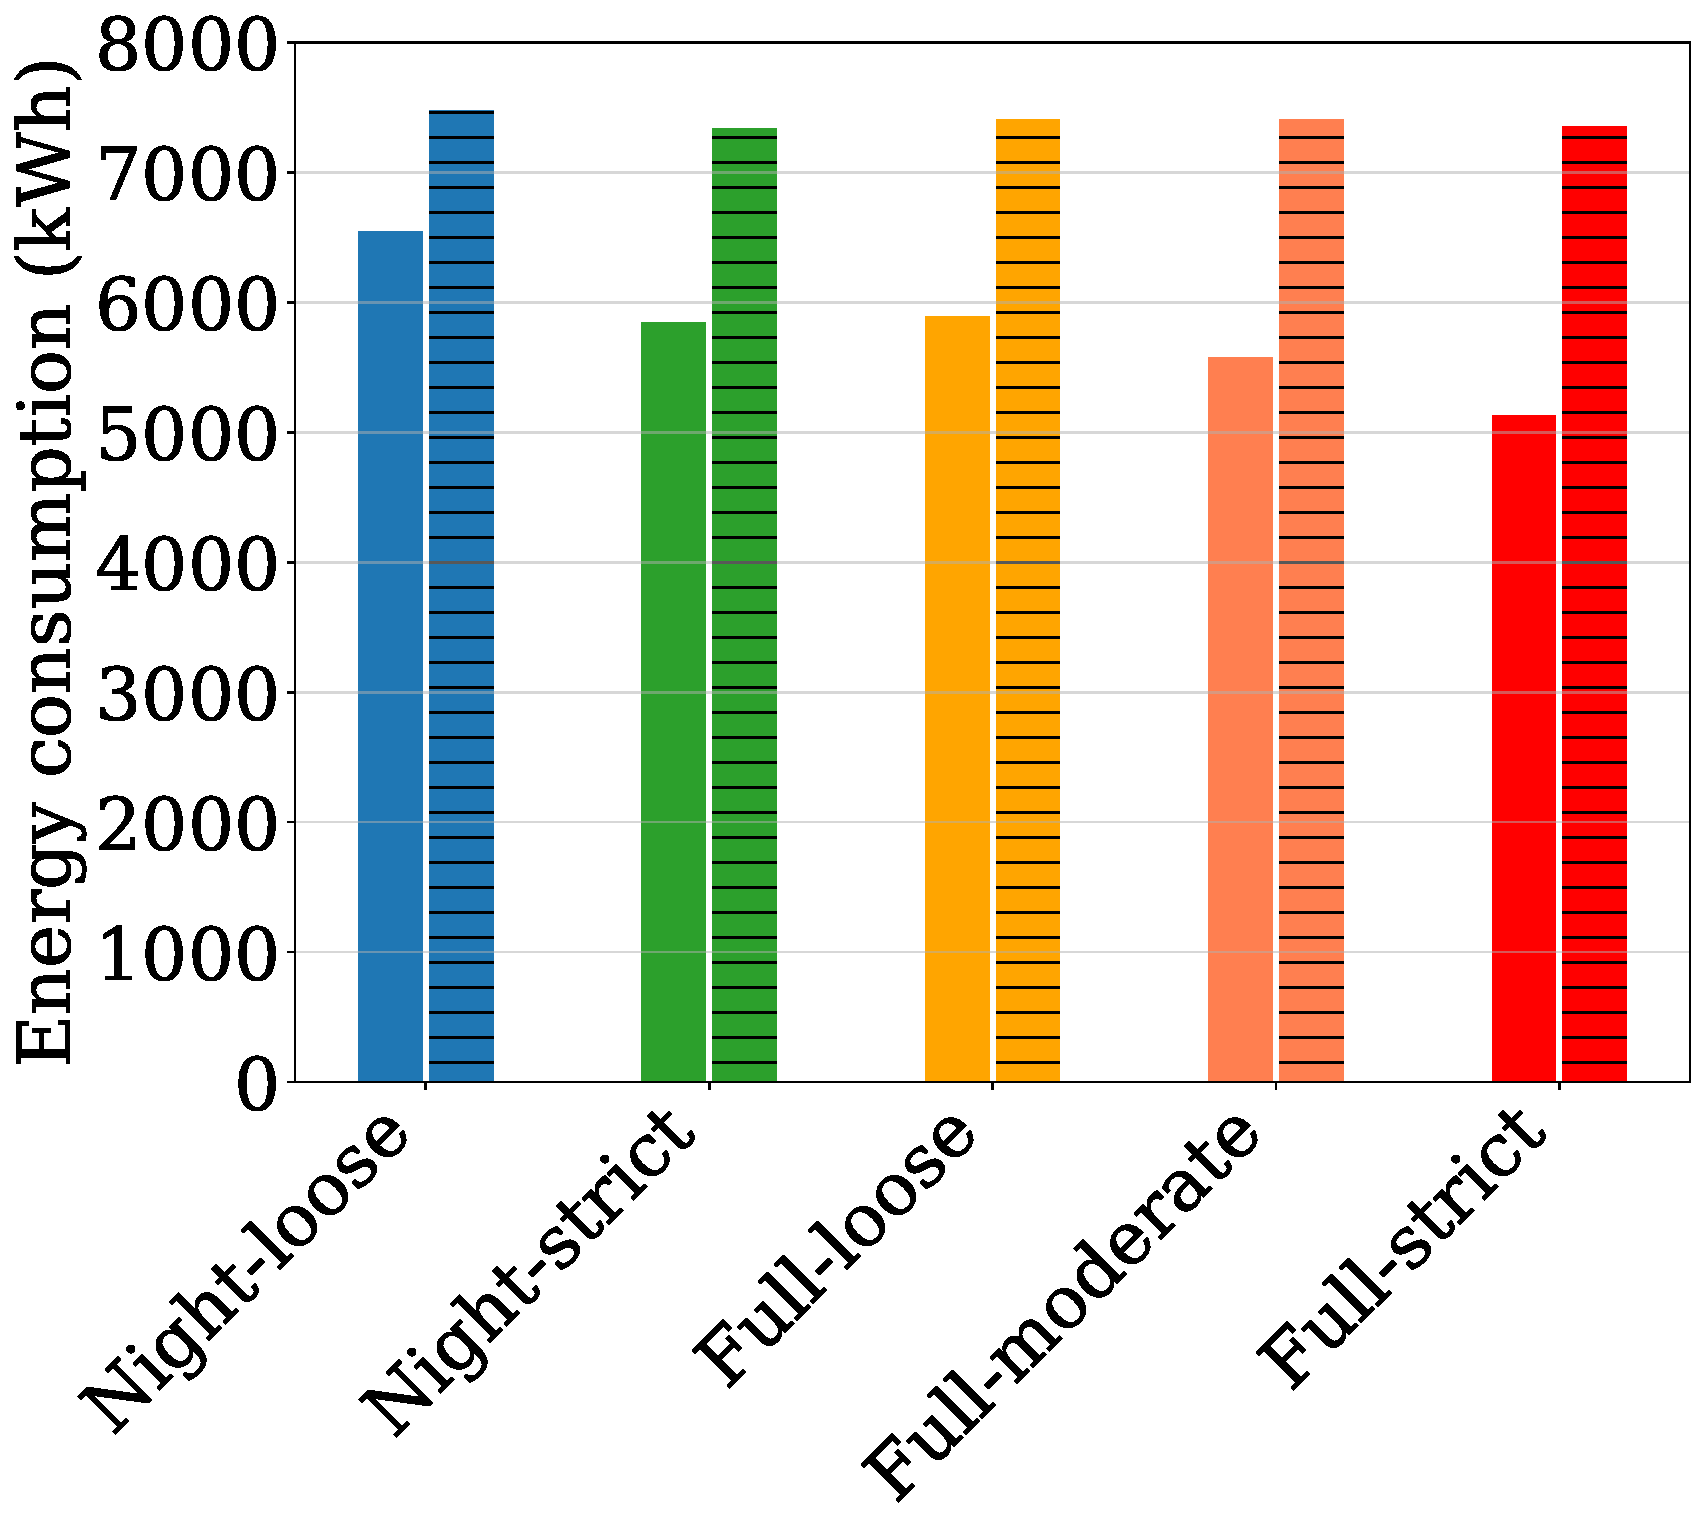
\includegraphics[width=.5\columnwidth]{images/energy/energy_saving/capacity_booster/energy_consumption_actual_and_benchmark_southeast.pdf}}
%     \caption{Total energy consumption of capacity booster and benchmark
%     \js{check confidentiality of energy consumption}
%     }\label{fig:total_energy_consumption_benchmark}
% \end{figure}


%As noted before, energy consumption depends on the traffic load; therefore, in order to properly estimate and compare the energy savings that each strategy offers, we need to account for the traffic variability across the weeks of the trials. 
%Indeed, there is variability of total traffic during the trials of between $3.2\%$ and $3.7\%$, which can be explained by holidays and social events that happen in the areas we target.
%Therefore, in order to avoid biasing the results, we propose to compare the actual energy consumption against a benchmark model that represents \textit{what would have been the energy consumption of the capacity cell if the energy-saving policy were not in place}. 
During the trial periods, we observed some variability in the aggregated traffic load in the two studied regions. These changes in the user traffic demand typically depend on external factors, such as local holidays and social or sports events. Specifically, we see a traffic variability of $3.2\%$ for the Dense region and $3.7\%$ for the Sparse region over the different weeks of the trials. Note that all strategies were tested for an entire week, which mitigates variability due to the difference in traffic between weekdays and weekends across the different strategies. To make a fair comparison, we take as a reference a model that represents a reverse trial, \ie~\textit{what would have been the energy consumption of cells in the absence of the energy saving strategies}. In this case capacity cells do not enter into cell sleep mode, hence the energy consumption model always accounts for the fixed circuit power $\gamma$ on all radio units, even if the cell load drops to zero. Conversely, in the tested strategies the model considers $E_{RRU}$=$0$ (\ie $\gamma$=$0$; $R_{PRB}$=$0$) when cells enter into sleep mode. This no-sleep configuration allows us to compare the various energy saving strategies in relative terms, reporting their percent saving with respect to a no-sleep scenario so that the results are robust to possible traffic load fluctuations over the trial periods.
%Now, with the corresponding benchmark in place, we can accurately obtain the corresponding energy saving, avoiding the difference in traffic load over the trials.

\begin{figure}
    \centering
    \subfloat{
    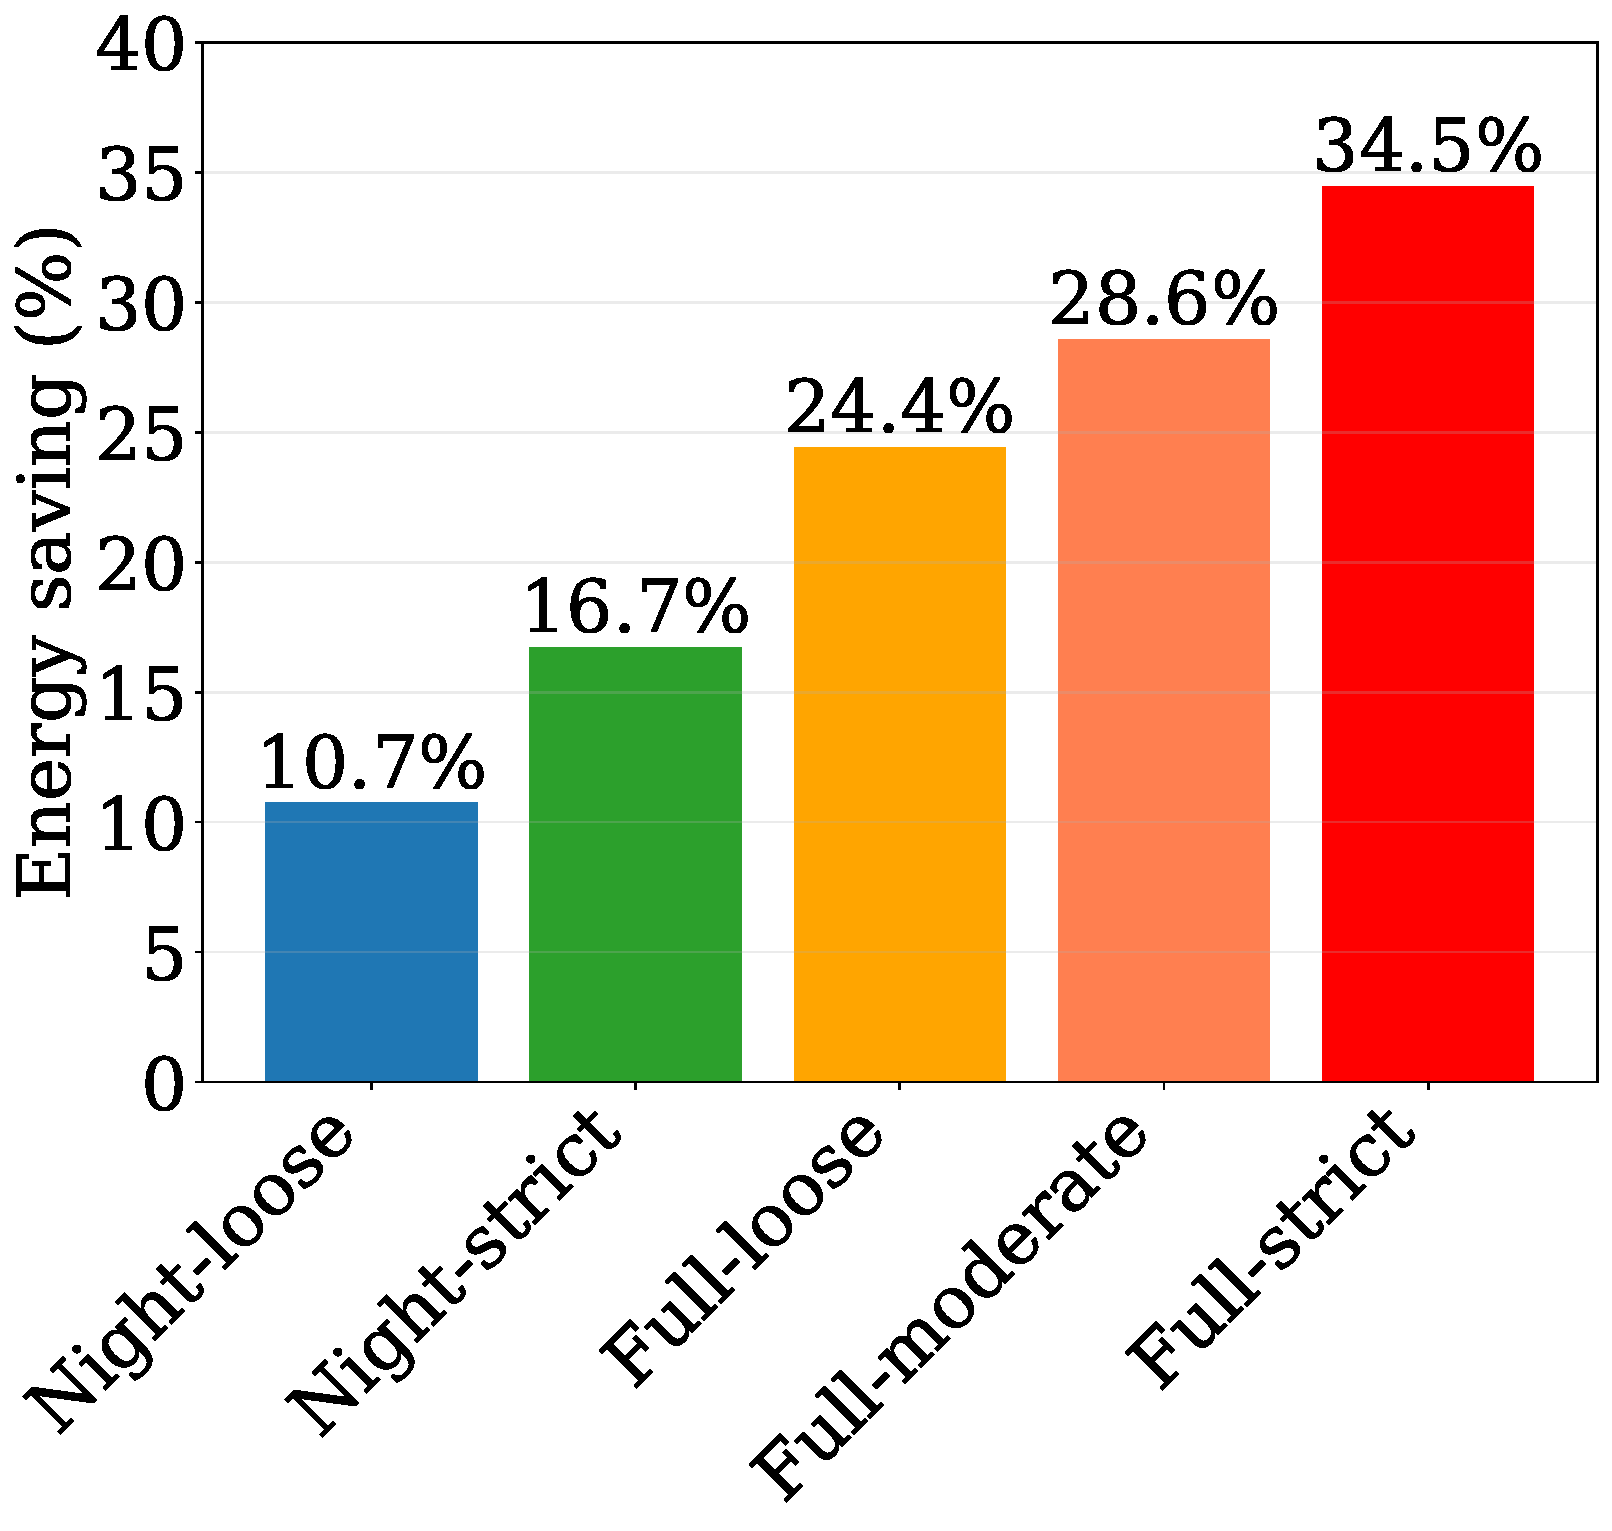
\includegraphics[width=.4875\columnwidth]{images/energy/energy_saving/capacity_booster/saving_percentage_north_london.pdf}}
    \subfloat{
    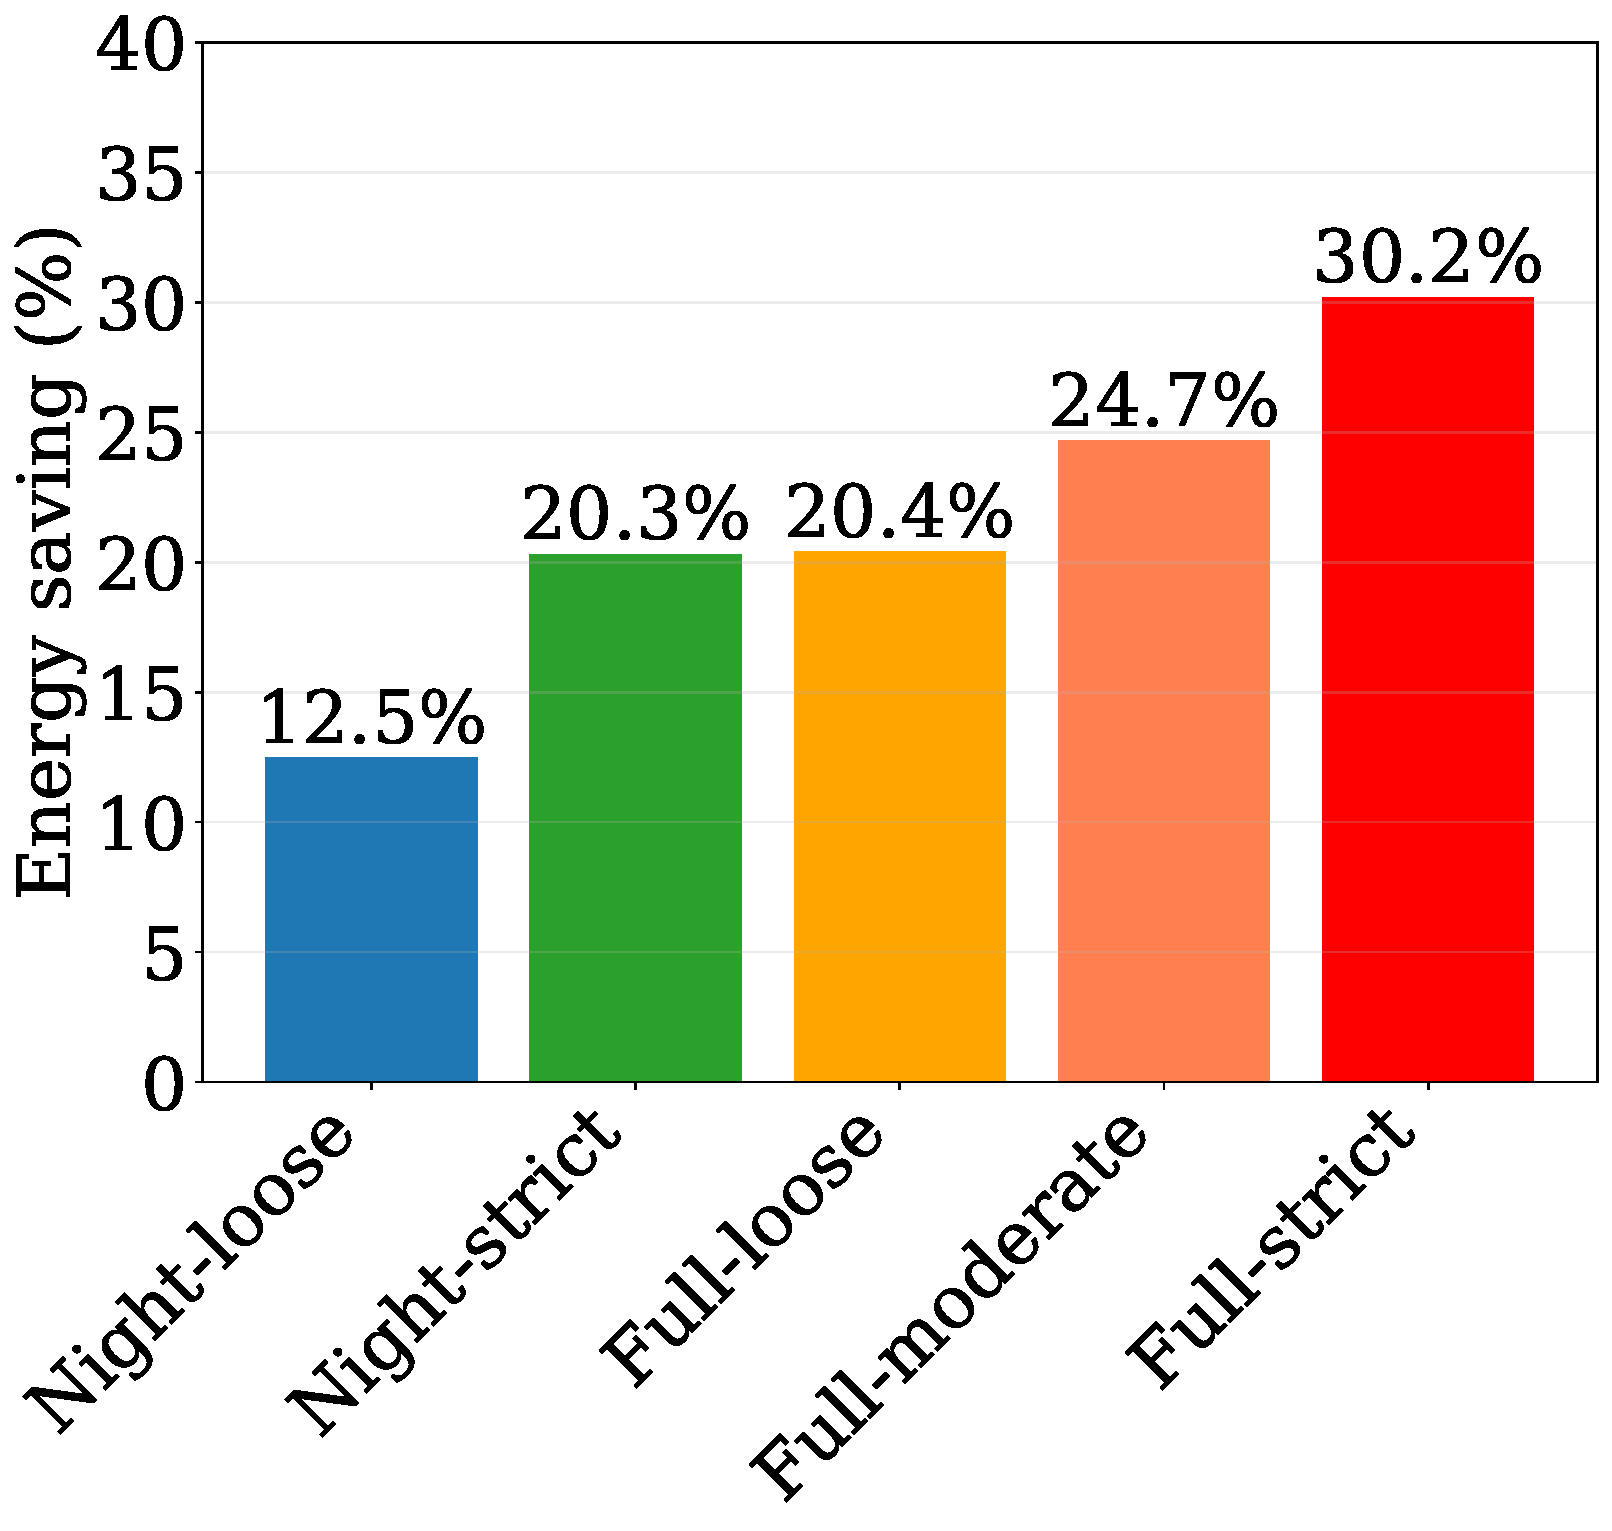
\includegraphics[width=.4875\columnwidth]{images/energy/energy_saving/capacity_booster/saving_percentage_southeast.pdf}}

    \centering
    \subfloat{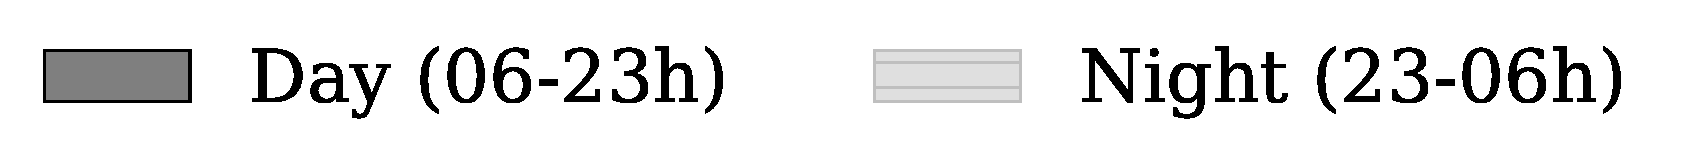
\includegraphics[width=.55\columnwidth]{images/energy/energy_saving/capacity_booster/saving_percentage_breakdown_boxplot_agg_frecuency_areas_legend.pdf}}
    
    \setcounter{subfigure}{0}

    \centering
    \subfloat[Dense region]{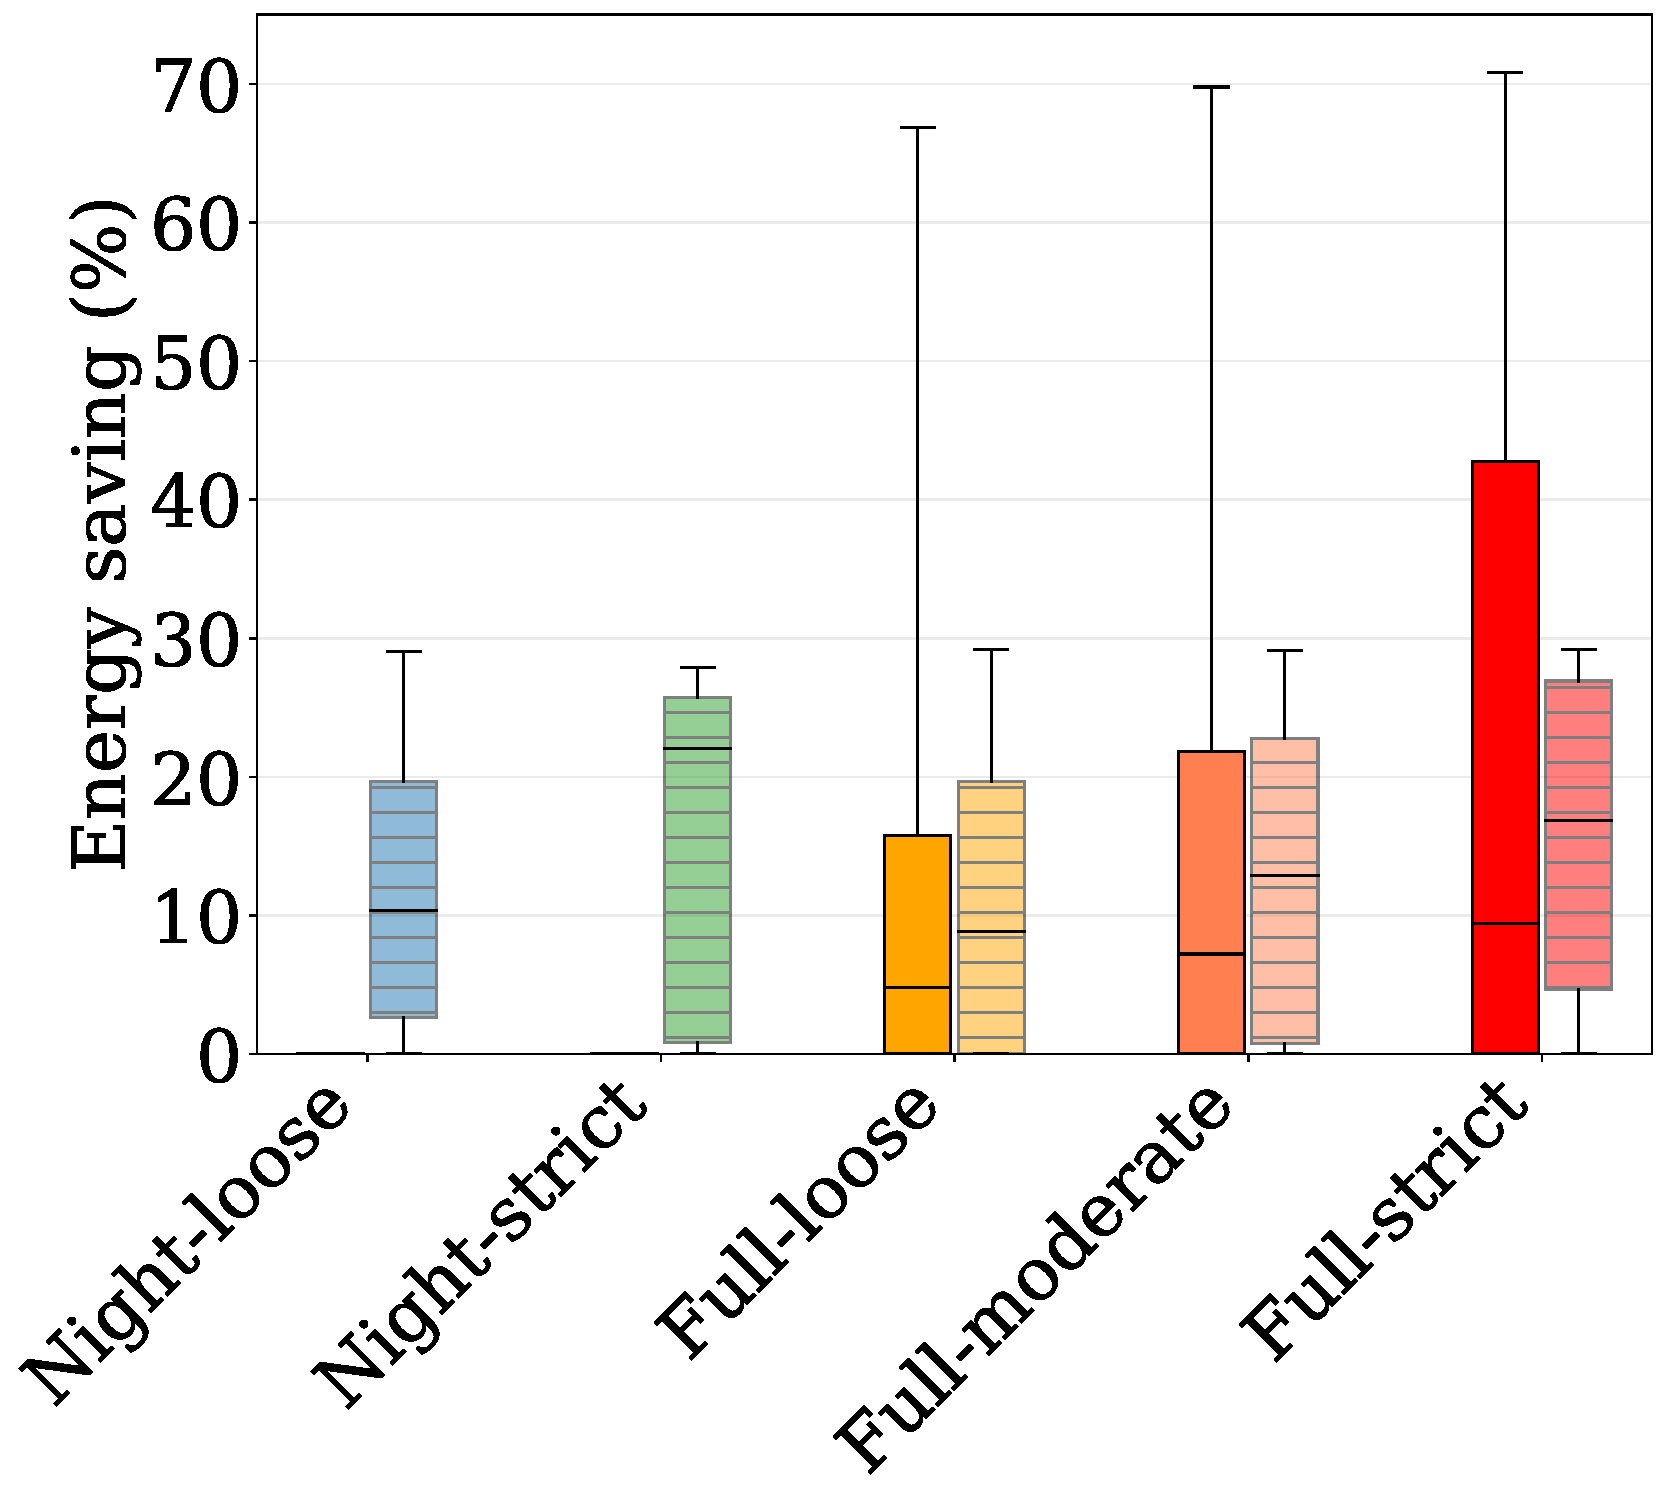
\includegraphics[width=.5\columnwidth]{images/energy/energy_saving/capacity_booster/saving_percentage_breakdown_boxplot_agg_frecuency_north_london.pdf}}
    \subfloat[Sparse region]{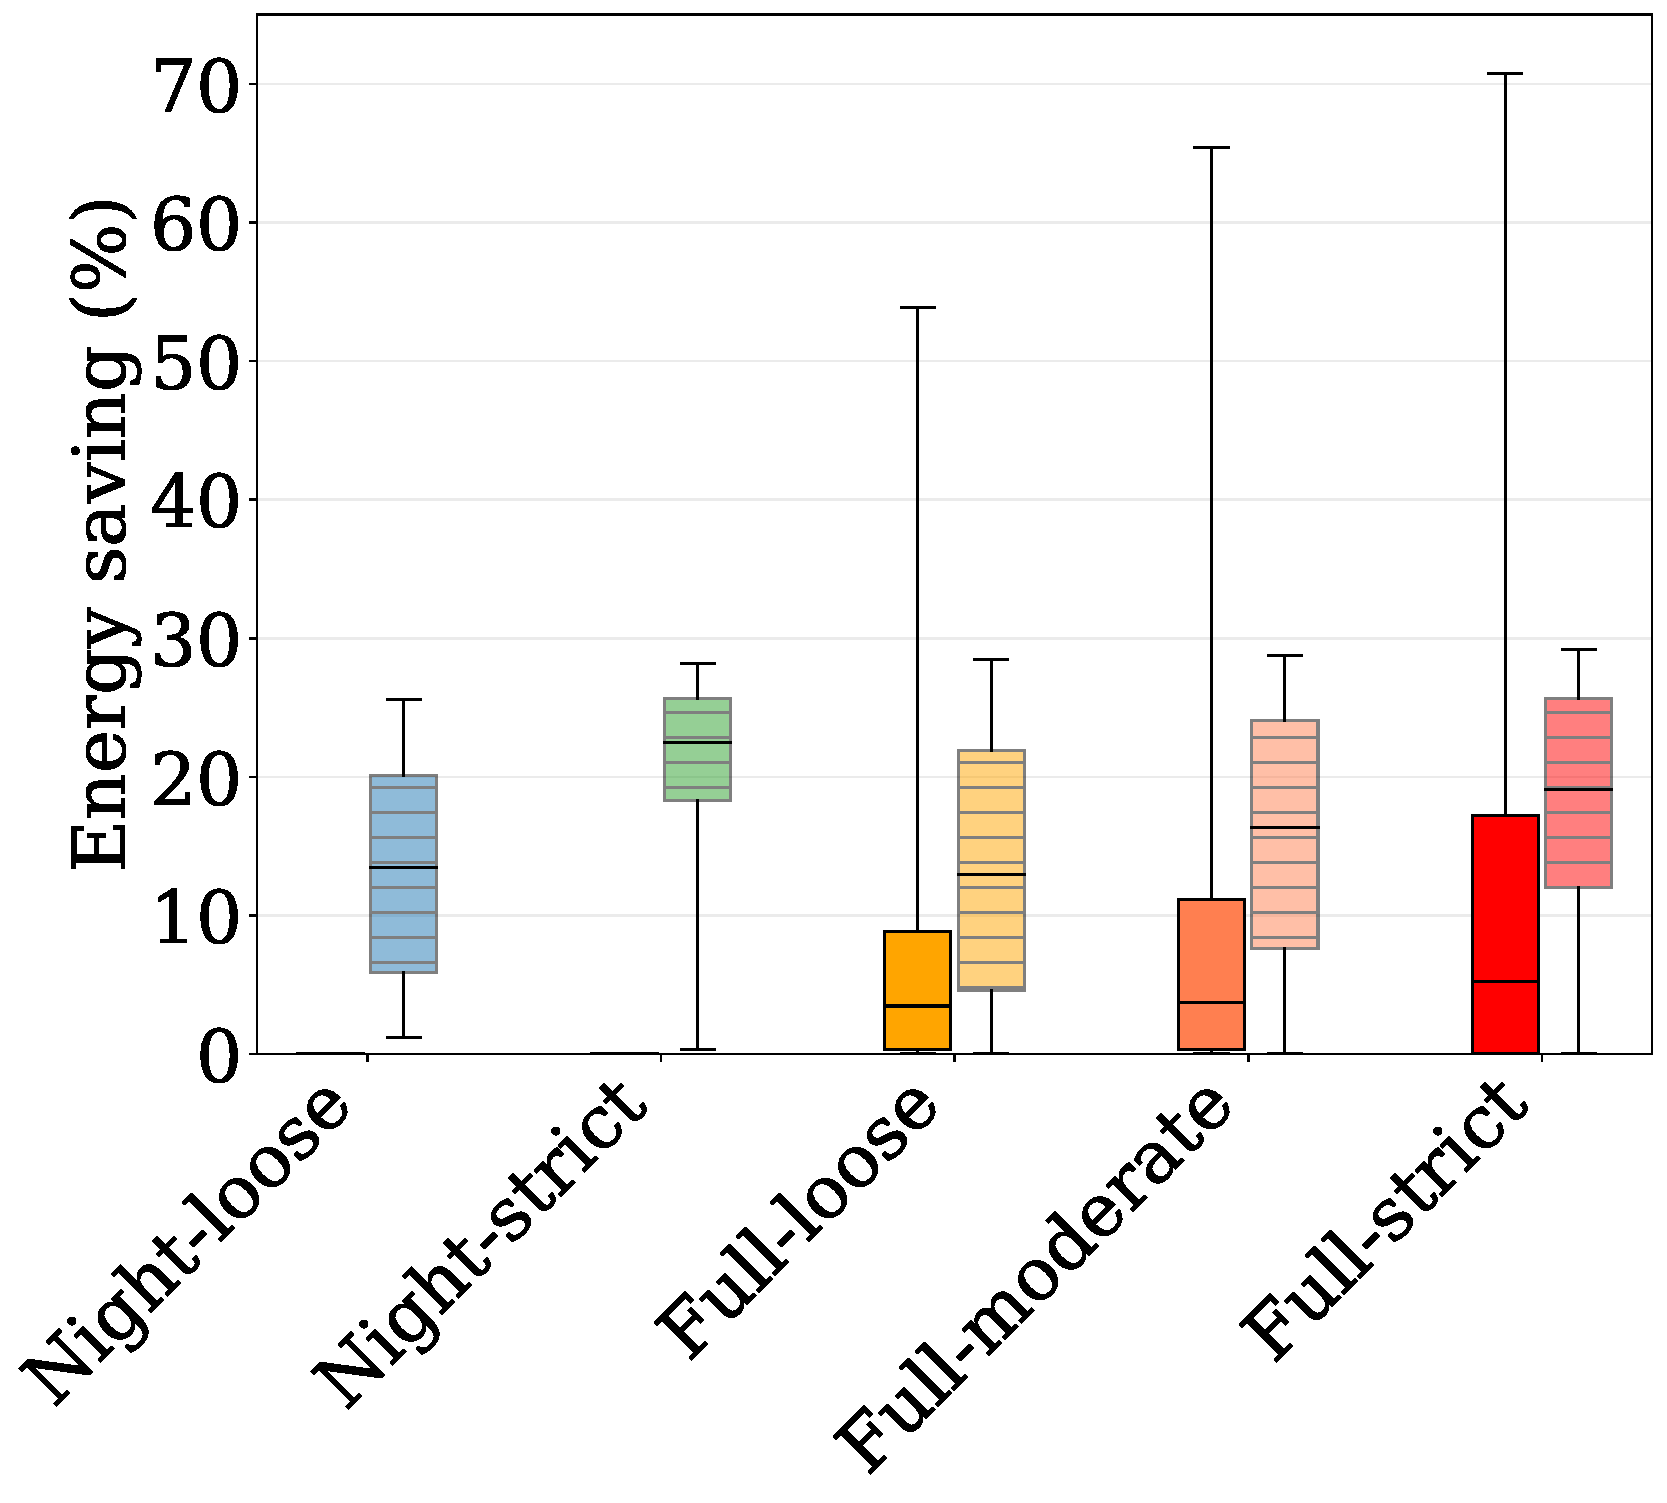
\includegraphics[width=.5\columnwidth]{images/energy/energy_saving/capacity_booster/saving_percentage_breakdown_boxplot_agg_frecuency_southeast.pdf}}
    \vspace{-4pt}
    \caption{\small 
    Top - Percentage of energy saving obtained by capacity cells in the two regions; Bottom - Distribution of energy savings over the capacity cells during day and night periods. 
    % \js{Can we add time intervals in the legend for "Day" and "night"?}
    }\label{fig:percentage_energy_saving_capacity_boosters}
    \vspace{-15pt}
\end{figure}

%As can be expected, policies that are in place for longer periods of time and with higher thresholds not only increase the time that cells are sleeping but also translate into lower energy consumption, with savings between $30\%$-$34\%$ in energy consumption with respect to a scenario where antennas do not switch off as shown in the top row of Figure~\ref{fig:percentage_energy_saving_capacity_boosters}. 

%An interesting question is to understand from which period of the day these savings are coming. In order to maintain consistency with the Night-loose and Night-strict strategies, we defined the nighttime period the same as these strategies, from 23:00 to 06:00, and the daytime as the rest of the time.
%The bottom row of Figure~\ref{fig:percentage_energy_saving_capacity_boosters} shows the distribution of energy saving per antenna over these portions of the day.
%A deeper inspection of the full kind policies reveals heterogeneous behavior where more than half $57-58\%$ of the savings in the Dense region came from cells sleeping during the day period, surprising in the Sparse region, the nighttime saving accounts for $55-60\%$ of the total savings. 
%The results suggest that increasing the activation time of the Night strategies may be enough to achieve the same savings produced in a full day.

% Figure~\ref{fig:percentage_energy_saving_capacity_boosters} (top plots) show the energy saving improvement with respect to the benchmark model (in \%) in the two regions. In general, all strategies exhibit significant energy savings, which are clearly correlated with the policy time windows (night vs full-day) and the ON/OFF thresholds that each strategy implements. The most aggressive Full-strict strategy exhibits an energy saving of $30.2\%$ and $34.5\%$ in the Dense and Sparse regions, respectively. To further investigate the behavior of these strategies along the day, we differentiate between energy savings during daytime (06-23h) and nighttime (23-06h). The nighttime coincides with the time window where Night-loose and Night-strict strategies are deployed. Figure~\ref{fig:percentage_energy_saving_capacity_boosters} (bottom plots) show the distributions of energy savings per cell over the two periods of time. The results reveal that most cells experience greater savings during the night (see median values), which is expected due to the lower traffic load during this time period. However, we observe an interesting behavior over daytime on full-day strategies: as the thresholds become higher (\ie~more aggressiveness) some cells start to experience significant energy savings. Despite the median cells during the night period achieve higher energy saving than during daytime, it is important to keep in mind that the day period considered is larger than the nighttime period; therefore, a deeper analysis reveals that these overall savings are achieved by $58.0\%$, $57.7\%$, and $58.0\%$ during daytime respectively for the Full-loose, Full-moderate, and Full-strict strategies in the Dense region, and $39.9\%$, $42.4\%$, and $44.9\%$ also during during daytime in the Sparse region. 
% These results suggest that some portions of the cells achieve savings during nighttime similar to those achieved during daytime, opening the door to speculate that increasing the activation time of the night strategies may be enough to achieve the same savings produced in a full day.

Figure~\ref{fig:percentage_energy_saving_capacity_boosters} (top) shows the energy-saving improvement with respect to the benchmark model (in \%) in the two regions. Overall, all strategies exhibit significant energy savings, which are clearly correlated with the policy time windows (night vs full-day) and the ON/OFF thresholds that each strategy implements. The most aggressive Full-strict strategy exhibits an energy saving of $34.5\%$ and $30.2\%$ in the Dense and Sparse regions, respectively. To further investigate the behavior of these strategies along the day, we differentiate between energy savings during daytime (06-23h) and nighttime (23-06h). The nighttime coincides with the time window where Night-loose and Night-strict strategies are deployed. 
Figure~\ref{fig:percentage_energy_saving_capacity_boosters} (bottom) shows the distributions of energy savings per cell over the two periods of time. The results reveal that most cells experience greater savings during the night (see median values), which is expected due to the lower traffic load during this time period.

However, we observe an interesting behavior over daytime on full-day strategies: as the thresholds become higher (\ie~more aggressiveness) some cells start to experience significant energy savings during this period. Although the median cells achieve similar energy savings across strategies over daytime, a portion of the cells experience considerably greater savings with more aggressive thresholds. Particularly, if we look at the saving of top-25\% cells during daytime (\ie~pct-75), these cells achieve savings of $15.8\%$ ($8.8\%$), $21.8\%$ ($11.2\%$), and $42.7\%$ ($17.2\%$) 
% \js{@Orlando: fill in these values}
for the Full-loose, Full-moderate, and Full-strict strategies, respectively, in the Dense (Sparse) regions. These results reveal that a considerable portion of the cells can achieve more energy savings during daytime than during the nighttime. Note that these results are subject to the definition of night period, which is 7 hours, and daytime, which extends over the remaining 17 hours in our case.